\documentclass[11pt,a4paper,sans,dvipsnames]{report}
%%%%%%%%%%%%%%%%%%%%%%%%%%%%%%%%%HEADER FROM ADRIAN SATIN, modified by william fabre %%%%%%%%%%%%%%%%%%%%%%%%%%%%%%%%%%%%%%
\usepackage[utf8]{inputenc} 
\usepackage{graphicx} % support the \includegraphics command and options
%\usepackage[frenchb]{babel}
\usepackage{tikz}
%*\usepackage{circuitikz}
\usetikzlibrary{circuits}
\graphicspath{{images/}}% chemin vers les images
\usepackage[parfill]{parskip} % Activate to begin paragraphs with an empty line rather than an indent
%%% PACKAGES
\usepackage{hyperref} % Gestion Hyperliens/url
% https://en.wikibooks.org/wiki/LaTeX/Hyperlinks
\usepackage{eurosym}
\usepackage{fancyhdr}
\usepackage{color}
\usepackage{svg}
% YOLO NICE CODE EXEMPLE merci axel
%\usepackage{minted}
%\usepackage{paralist} % very flexible & customisable lists (eg. enumerate/itemize, etc.)
%\usepackage{verbatim} % adds environment for commenting out blocks of text & for better verbatim
\usepackage{subfig} % make it possible to include more than one captioned figure/table in a single float
\usepackage{graphicx}
\usepackage{fancyhdr}
\usepackage{multicol}
\usepackage{listings}
\usepackage{amsmath,amsfonts,amsthm,amssymb}
\usepackage{pdfpages}
\usepackage{comment}
\usepackage{caption}
\definecolor{violet-logo}{RGB}{23,63,28}
%%% HEADERS & FOOTERS
\usepackage{fancyhdr} % This should be set AFTER setting up the page geometry
\pagestyle{plain} % options: empty , plain , fancy
\renewcommand{\headrulewidth}{1pt} % customise the layout...
\lfoot{}\cfoot{\thepage}\rfoot{}
%%% SECTION TITLE APPEARANCE
%*\usepackage{sectsty}
\allsectionsfont{\sffamily\mdseries\upshape} % (See the fntguide.pdf for font help)
% (This matches ConTeXt defaults)
%%% ToC (table of contents) APPEARANCE
\usepackage[nottoc,notlof,notlot]{tocbibind} % Put the bibliography in the ToC
%*\usepackage[titles,subfigure]{tocloft} % Alter the style of the Table of Contents
\renewcommand{\cftsecfont}{\rmfamily\mdseries\upshape}
\renewcommand{\cftsecpagefont}{\rmfamily\mdseries\upshape} % No bold!
\usepackage{geometry} % to change the page dimensions
\geometry{left=2cm, right=2cm, bottom= 1cm}
\geometry{a4paper} % or letterpaper (US) or a5paper or....
\fancyhead{}
%%% END Article customizations

%nice chapter
\usepackage{titlesec}
\titleformat{\chapter}[display]
{\normalfont\bfseries}{}{0pt}{\Large}
\titlespacing*{\chapter}{0pt}{-50pt}{40pt}

% nice section
\makeatletter
\def\@seccntformat#1{%
	\expandafter\ifx\csname c@#1\endcsname\c@section\else
\csname the#1\endcsname\quad
  \fi}
\makeatother

\usepackage{array,multirow,makecell}
\setcellgapes{1pt}
\makegapedcells
\newcommand{\HRule}{\rule{\linewidth}{0.5mm}} % Defines a new command for the horizontal lines, change thickness here
\fancyhf{} % sets both header and footer to nothing
\renewcommand{\headrulewidth}{0pt}
\addtolength{\topmargin}{-60pt}

%bibtex
\bibliographystyle{plain}

% defining my own style for code
%\usepackage{xcolor}
\usepackage[dvipsnames]{xcolor}
\definecolor{codegreen}{rgb}{0,0.6,0}
\definecolor{codegray}{rgb}{0.5,0.5,0.5}
\definecolor{codepurple}{rgb}{0.58,0,0.82}
\definecolor{backcolour}{rgb}{0.95,0.95,0.92}

\lstdefinestyle{mystyle}{
	%basicstyle=\fontsize\tiny\ttfamily %proper font size
	%basicstyle=\small, %or \small or \footnotesize etc.
	backgroundcolor=\color{backcolour},   
	commentstyle=\color{codegreen},
	keywordstyle=\color{magenta},
	numberstyle=\tiny\color{codegray},
	stringstyle=\color{codepurple},
	basicstyle=\ttfamily\footnotesize,
	breakatwhitespace=false,         
	breaklines=true,                 
	captionpos=t,                    
	keepspaces=true,                 
	numbers=left,                    
	numbersep=5pt,                  
	showspaces=false,                
	showstringspaces=false,
	showtabs=false,                  
	tabsize=2
}

\lstset{style=mystyle}


% my own command to add caption to figure code
\newcommand{\mylisting}[2][]{%
	\lstinputlisting[caption={\texttt{\detokenize{#2}}},#1]{#2}%
}



\begin{document}
\begin{titlepage}

	\center % Center everything on the page

	%----------------------------------------------------------------------------------------
	%	HEADING SECTIONS
	%----------------------------------------------------------------------------------------

	\textsc{\LARGE University Pierre et Marie Curie}\\[1.5cm] % Name of your university/college
	\textsc{\Large project MOCCA}\\[0.5cm] % Major heading such as course name

	%----------------------------------------------------------------------------------------
	%	TITLE SECTION
	%----------------------------------------------------------------------------------------
	\vfill
	\HRule \\[0.4cm]
	{ \huge \bfseries Report MOCCA : Synthesys, place and route of a given MIPS architecture with CADENCE toolchain}\\[0.4cm] 
	\HRule \\[1.5cm]
	\vfill
	%----------------------------------------------------------------------------------------
	%	AUTHOR SECTION
	%----------------------------------------------------------------------------------------

	\begin{minipage}{0.4\textwidth}
		\begin{flushleft} \large
			\emph{Authors:}\\
			% Ordre alphabetique sur les noms
			\textsc{Youcef Sekouri, William Fabre} 
		\end{flushleft}
	\end{minipage}
	~
	\begin{minipage}{0.4\textwidth}
		\begin{flushright} \large
			\emph{Teachers :} \\
			Mr \textsc{Matthieu Tuna},\textsc{Pirouz Bazarghan-Sabet}
		\end{flushright}
	\end{minipage}\\[2cm]

	%----------------------------------------------------------------------------------------
	%	DATE SECTION
	%----------------------------------------------------------------------------------------

	{\large Year 2019-2020}\\[2cm] % Date, change the \today to a set date if you want to be precise

\end{titlepage}

\newpage
\tableofcontents
\vspace*{3cm}
\begingroup\let\clearpage\relax

	\newpage
	\chapter{Project script RTL compiler}
	This is our script, it has been inspired by this source\footnote{\url{https://sudip.ece.ubc.ca/rtl-compiler/}}
	\lstinputlisting[language=bash]{../src/script.tcl}





	\newpage
	\chapter{RTL Compiler}


	% https://vlsiuniverse.blogspot.com/2016/12/liberty-format-introduction.html
	% http://vlsiuniverse.blogspot.in/2014/07/propagation-delay.html
	% https://vlsiuniverse.blogspot.com/search/label/cell%20delay
	% https://vlsispace.com/2019/10/01/cell-delay-of-standard-cell-and-what-are-the-facotors-effecting-the-cell-delay/
	\section{Load the libraries}

	Definition Liberty Timing File (LIB) : The .lib file is an \texttt{ASCII} format file that represents timing and power parameters associated with cells in a particular semiconductor technology. They are gathered by simulating the cells under various conditions. It can have multiple information\footnote{https://www.csee.umbc.edu/~tinoosh/cmpe641/, Liberty Timing File courses} :

	\begin{itemize}
		\item operating conditions such as temperature and voltage.
		\item fanout, capacitance, slew and all necessary thresholds.
		\item Lookup table for timing arcs, those are functions of output load capacitance and input slew.
		\item Area of the cell.
	\end{itemize}

	\subsection*{Explain the difference between these two different types.}
	\begin{itemize}
		\item The Library MAX (worst case) is used to verify the stability of the signal before the edge, also called setup time violation.
		\item The Library MIN (best case) is used to verify the stability of the signal after the edge, also called hold time violation.
	\end{itemize}


	\subsection*{Which one is needed for the synthesis step ? Explain your choice.}
	During synthesis stage we only have a bunch of cells without any routing delays between them. However, we still have for each cells, timing aspects:



	\begin{itemize}
		\item Rise Delay (Cell Rise): Propagation delay between output and input when output changes from 0 to 1.
		\item Fall Delay (Cell Fall): Propagation delay between output and input when output changes from 1 to 0.
		\item The threshold points from which 0 goes to 1 or 1 goes to 0 for the input and for the output.
		\item Rise Slew (Rise Transition):
			\begin{itemize}
				\item lower slew threshold: Threshold from which it is considered to go to 1.
				\item upper slew threshold: Threshold from which it is considered to be 1.
			\end{itemize}
		\item Fall Slew (Fall Transition):
			\begin{itemize}
				\item upper slew threshold: Threshold from which it is considered to go to 0.
				\item lower slew threshold: Threshold from which it is considered to be 0.
			\end{itemize}
	\end{itemize}


	\begin{figure}[h!]
		\centering
		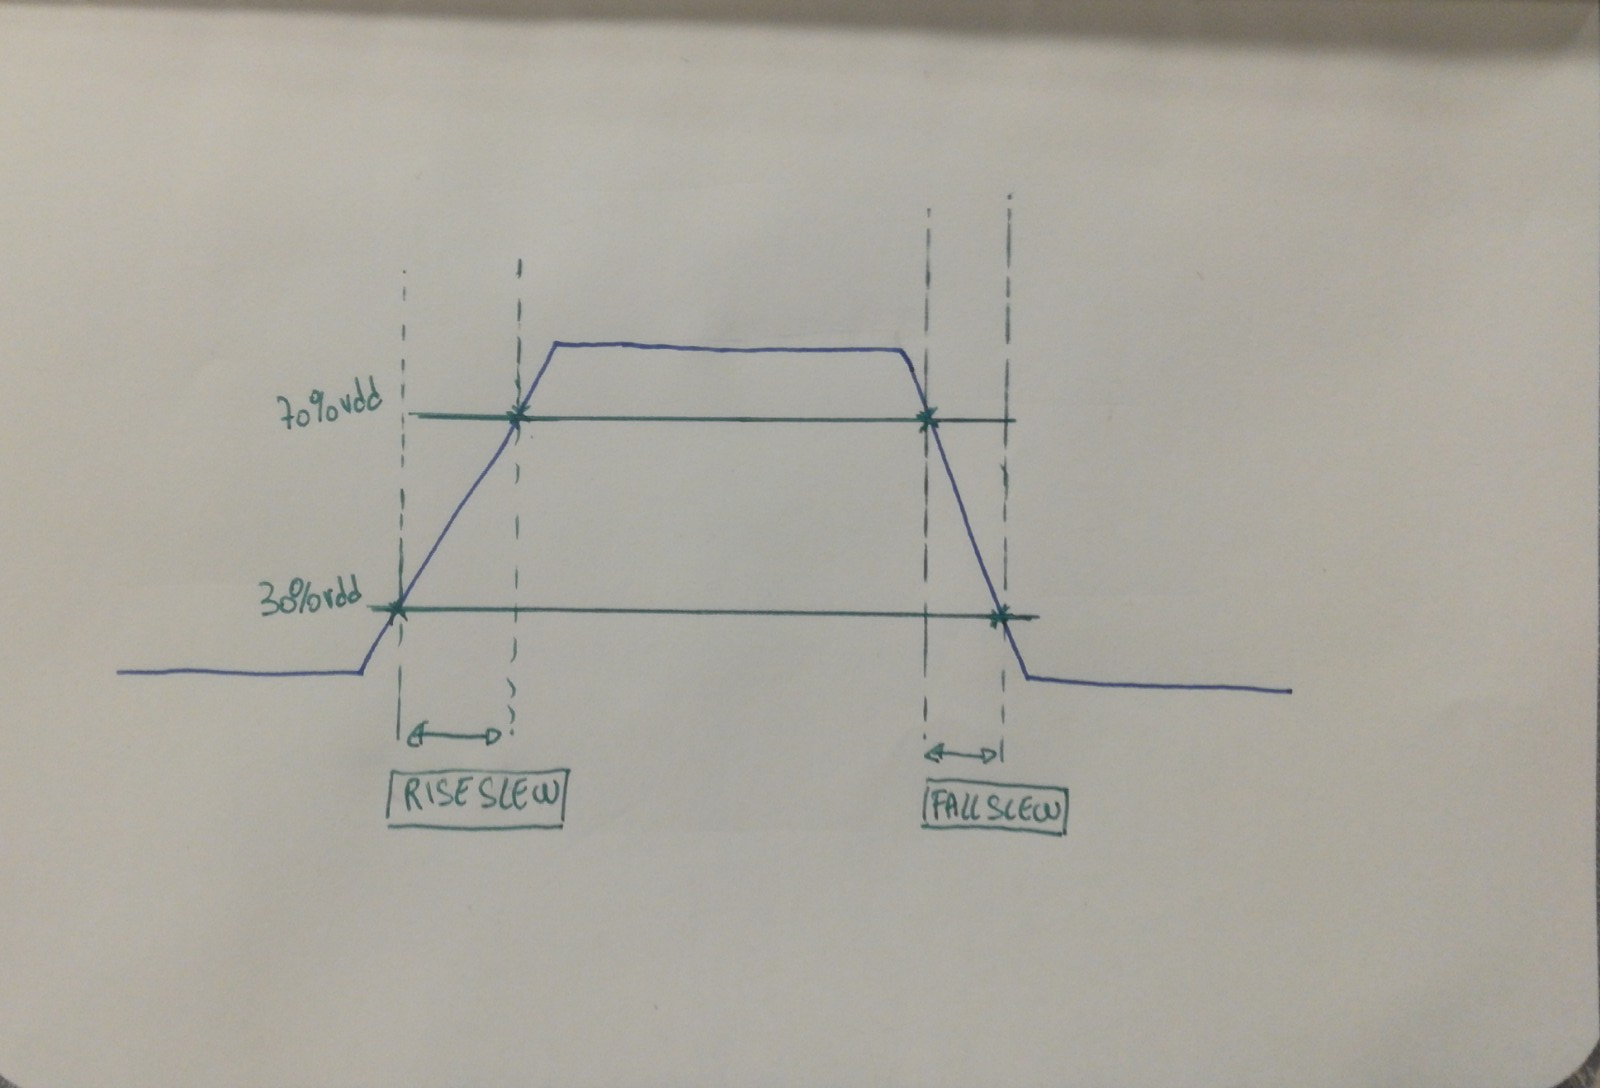
\includegraphics[width=.65\linewidth, frame]{images/slew.jpg}
		\captionof{figure}{Representation of an imaginary gate slews if the lower and upper threshold are respectively 30\% and 70\% for the fall and the rise}
		\label{fig:slew}
	\end{figure}%

	\begin{figure}[h!]
		\centering
		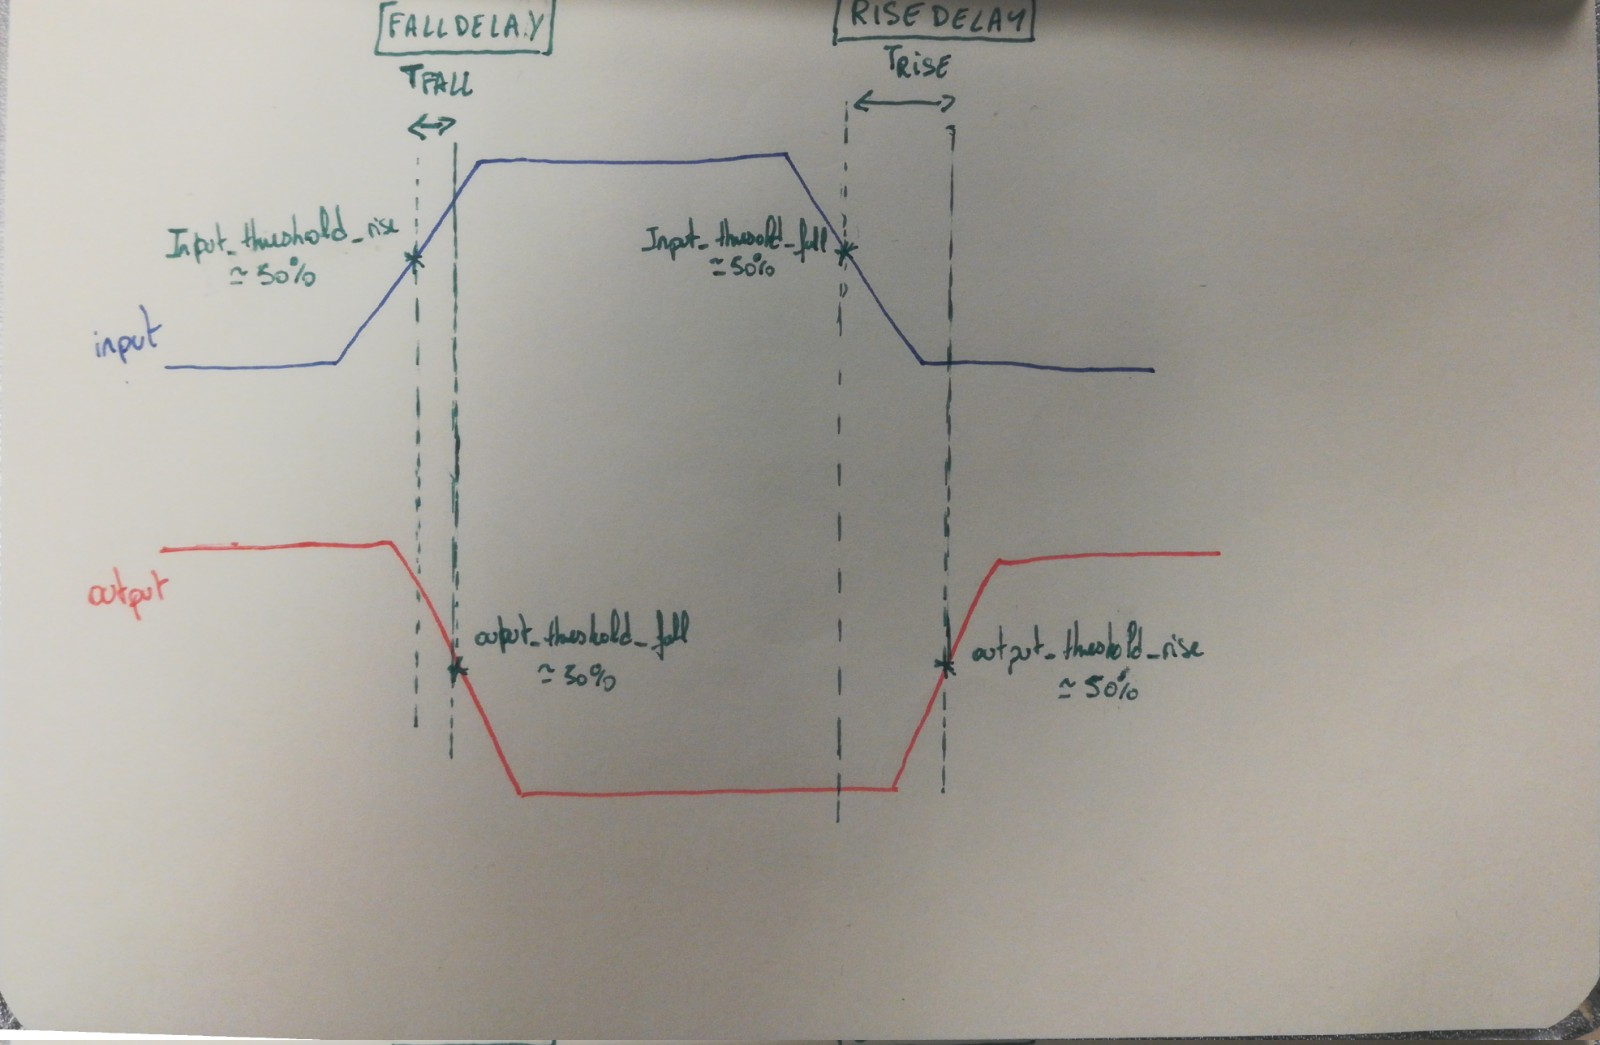
\includegraphics[width=0.65\linewidth, frame]{images/delay.jpg}
		\captionof{figure}{Representation of the Fall Delay and the Rise Delay of an imaginary inverter gate, in blue the input, in red the output.}
		\label{fig:delay}
	\end{figure}

	Therefore, we can use the WC library during the synthesis phase to check if we meet the setup requirements. The sum of delays of a long path of gates can create a setup time violation.
	The hold time violation is a shortest path problem on the clock tree, here we don't have any clock tree.
	Furthermore, we can use statistical models (Wire Load Model) which will allow us to do a more coherent timing analysis during synthesis. 

	\newpage
	\subsection*{Pick up a timing arc in the WC lib and the same timing arc in the BC, what is the value in the first library and in the second library. Add in your report a figure of the cell and the corresponding timing arc.}

	Here are some interesting differences between WC lib and BC lib to know before we watch the graphics. Values for Temperature and Voltage:


	\newpage
	\begin{figure}[h!]
		\centering
		\begin{tabular}{lllll}
			\cline{1-3}
			\multicolumn{1}{|l|}{}                    & \multicolumn{1}{l|}{WC lib} & \multicolumn{1}{l|}{BC lib} &  &  \\ \cline{1-3}
			\multicolumn{1}{|l|}{nominal Voltage}     & \multicolumn{1}{l|}{1,08}   & \multicolumn{1}{l|}{1,32}   &  &  \\ \cline{1-3}
			\multicolumn{1}{|l|}{nominal Temperature} & \multicolumn{1}{l|}{0}      & \multicolumn{1}{l|}{125}    &  &  \\ \cline{1-3}
		\end{tabular}
		\captionof{figure}{Table of nominal Voltage and Temperature for WC and BC lib.}
		\label{fig:table}
	\end{figure}%

	\begin{figure}[h!]
		\centering
		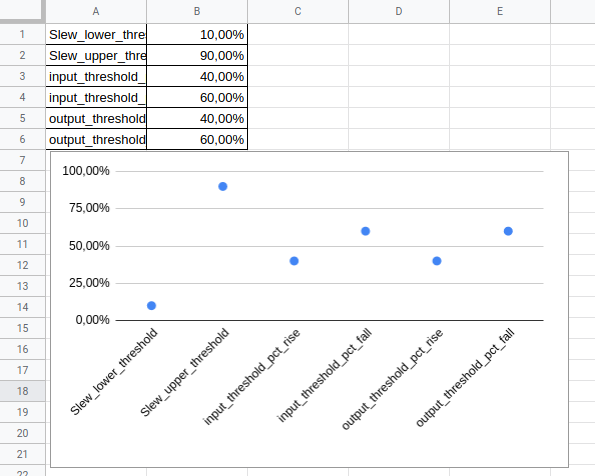
\includegraphics[width=.57\linewidth, frame]{images/slew_graph.png}
		\captionof{figure}{Representation of all the necessary thresholds to characterize the cell for both WC and BC (same results), slew, input, output.}

		\label{fig:slew_graph}
	\end{figure}%

	\begin{figure}[h!]
		\centering
		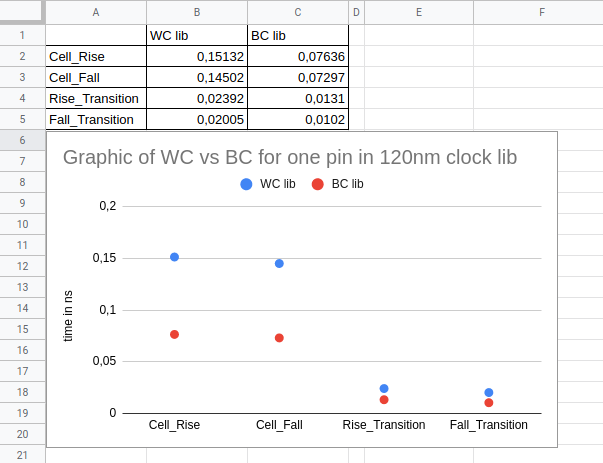
\includegraphics[width=0.57\linewidth, frame]{images/delay_graph.png}
		\captionof{figure}{Representation of the Fall Delay, the Rise Delay, Rise Slew, Fall Slew, we can clearly see a difference between the WC and BC library.}
		\label{fig:delay_graph}
	\end{figure}

	\newpage
	%https://books.google.fr/books?id=PCLfT7pxogMC&pg=PA157&dq=elaborate+vlsi&hl=fr&sa=X&ved=0ahUKEwiA8sfg-t_nAhVKJBoKHTY3D7oQ6AEIKTAA#v=onepage&q=elaborate%20vlsi&f=false
	%https://forums.xilinx.com/t5/Synthesis/what-exactly-is-elaborating-a-design/td-p/682043
	\section{Elaborate}
	\subsection*{The "elaborate" step does not synthesize the design, we will synthesize the design later on. What
		is the difference between elaboration and synthesis ?}

	From this link there is a clear definition of elaboration a design\footnote{\url{https://forums.xilinx.com/t5/Synthesis/what-exactly-is-elaborating-a-design/td-p/682043}}.

	Synthesis might be seen as one big step for a user perspective. It consists of :

	\begin{itemize}
		\item Elaborating the design.
		\item Apply constraints to the design.
		\item High level optimizations of the design.
		\item technology mapping (mapping with the library).
		\item Low level optimizations of the design.
	\end{itemize}

	\par The Elaborate step consists is reading RTL file to recognize hardware structures and transform them into future placeholders for the technology mapping. 
	\par It seems that for some tools, the elaborate step also do some syntax checks and verify the connections between structure. For example if two outputs are connected etc.
	\par This step is crucial because you cannot apply constraints on an RTL file, so those placeholders will be the premises of our netlist.


	\begin{figure}[h!]
		\centering
		\begin{lstlisting}
			rc:/> elab -h
			elaborate: elaborates previously read HDL files and creates corresponding design and subdesigns.
		\end{lstlisting}
		\captionof{figure}{Help option from RC interpreter.}
		\label{fig:rc_elaborate}
	\end{figure}




	\newpage
	\section{Check Design}
	%https://www.csee.umbc.edu/~tinoosh/cmpe641/tutorials/rc/rc_commandref.pdf
	%https://support1.cadence.com/public/docs/content/20417373.html
	%https://sudip.ece.ubc.ca/rtl-compiler/
	\subsection*{Is everything OK ? Please explain what are the problems. The most important one is the
		'Unresolved References', what is a missing the model ?}

	Definition of check\_design command : "Provides information on undriven and multi-driven ports and pins, unloaded sequential elements and ports, unresolved references, constants connected ports and pins, any assign statements and preserved instances in the given design. In addition, the command can report any cells that are not in both .lib and the physical libraries (LEF files).By default, if you do not specify an option, the check\_design command reports a summary table with this information."\footnote{\url{https://www.csee.umbc.edu/~tinoosh/cmpe641/tutorials/rc/rc_commandref.pdf} page 316}

	\par An unresolved Reference is when during the elaborate step, we go from vhdl to design, "undefined modules and VHDL entities are labeled “unresolved” and treated as blackboxes"\footnote{\url{https://www.csee.umbc.edu/~tinoosh/cmpe641/tutorials/rc/rc_commandref.pdf}, p284}.

	\begin{figure}[h!]
		\centering
		\begin{lstlisting}
			rc:/> check_design -unresolved  
			Checking the design.

			Unresolved References & Empty Modules
			------------------------------------- 
			No unresolved references in design 'MIPS_32_1P_MUL_DIV'

			No empty modules in design 'MIPS_32_1P_MUL_DIV'

			Done Checking the design.
		\end{lstlisting}
		\captionof{figure}{Example of check\_design usage on our design.}
		\label{fig:rc_elaborate}
	\end{figure}

	\par A missing model error seems to be when there is no IP it's a report that the cells are not in .lib nor in the physical libraries (LEF files).


	\newpage
	%TODO https://www.csee.umbc.edu/~tinoosh/cmpe641/slides/pipelining.pdf
	%EXPLICATIONS SUR LE PIPELINING DU RESET


	\section{Reset synchronizer}
	%https://www.researchgate.net/publication/228905230_Asynchronous_synchronous_reset_design_techniques-part_deux

	\subsection*{ What kind of reset is used in this design ? Synchronous or asynchronous ?}
	\par As we can see in the design the reset is asynchronous. Indeed, it is just a signal that comes from outside of the rtl design.

	\begin{figure}[h!]
		\centering
		\lstinputlisting[language=Vhdl, linerange={30-72}]{../src/mips_32_1p_mul_div.vhd}
		\captionof{figure}{RTL design interface, as we can see the second signal is the external reset.}
		\label{fig:sync_synchronizer}
	\end{figure}

	\newpage
	\subsection*{
		What is a reset synchronizer, please explain why a circuit should have a reset synchronizer ?
		Please explain the differences between both?
		Add TO your report the figure and the waveforms of your reset synchronizer.
	}
	It is use to synchronize an external reset with the clock domain of IC and do to prevent hold/set up violation.
	Indeed, the release of an external reset can happen asynchronously. So, reset must be synchronized to prevent meta-stability problem.
	There are two types of reset synchronizer : \\
	\begin{itemize}
		\item Asynchronous : The output signal activation is done asynchronously.
		\item Synchronous : The output signal activation is done synchronously.
	\end{itemize}
	The output signal deactivation, is always done synchronously.\\

	\subsection*{Synchronous Reset synchronizer}
	\begin{figure}[h!]
		\centering
		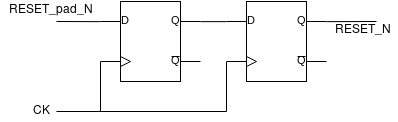
\includegraphics[width=0.65\linewidth]{images/sync_reset_sync.png}
		\captionof{figure}{A synchronous reset synchronizer}
		\label{fig:sync_synchronizer}
	\end{figure}

	\begin{figure}[h!]
		\centering
		\lstinputlisting[language=Vhdl, linerange={1-11}]{../src/reset_synchronizer_model.vhd}
		\captionof{figure}{VHDL example of a synchronous reset  synchronizer}
		\label{fig:sync_synchronizer_code}
	\end{figure}


	\begin{figure}[h!]
		\centering
		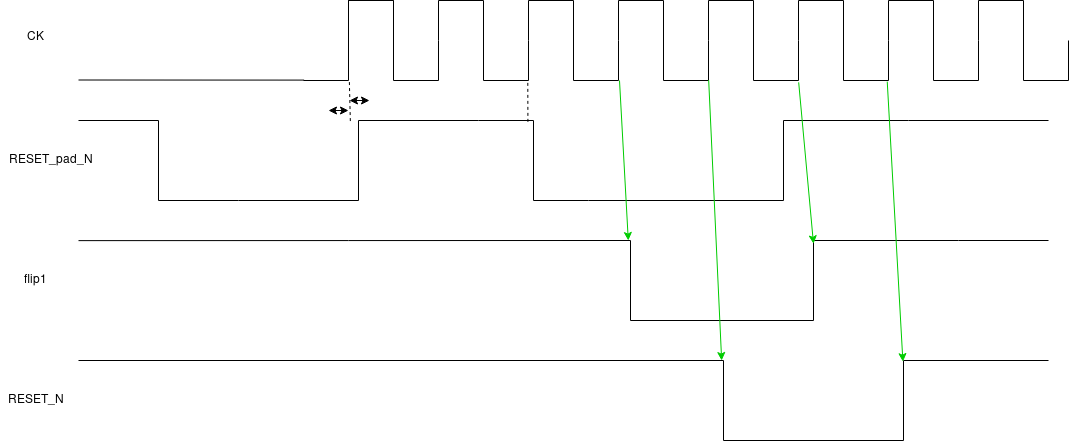
\includegraphics[height=0.32\linewidth,width=1.0\linewidth]{images/sync_reset_chrono.png}
		\captionof{figure}{Waveform of a synchronous reset synchronizer}
		\label{fig:sync_synchronizer_chrono}
	\end{figure}

	\newpage
	\subsection*{Asynchronous Reset synchronizer}
	\begin{figure}[h!]
		\centering
		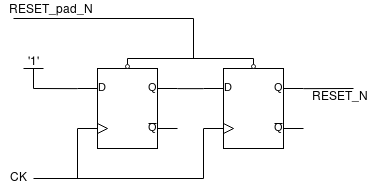
\includegraphics[width=0.65\linewidth]{images/async_reset_sync.png}
		\captionof{figure}{An asynchronous reset synchronizer}
		\label{fig:async_synchronizer}
	\end{figure}

	\begin{figure}[h!]
		\centering
		\lstinputlisting[language=Vhdl, linerange={13-26}]{../src/reset_synchronizer_model.vhd}
		\captionof{figure}{VHDL example of an asynchronous reset synchronizer}
		\label{fig:async_synchronizer_code}
	\end{figure}

	\begin{figure}[h!]
		\centering
		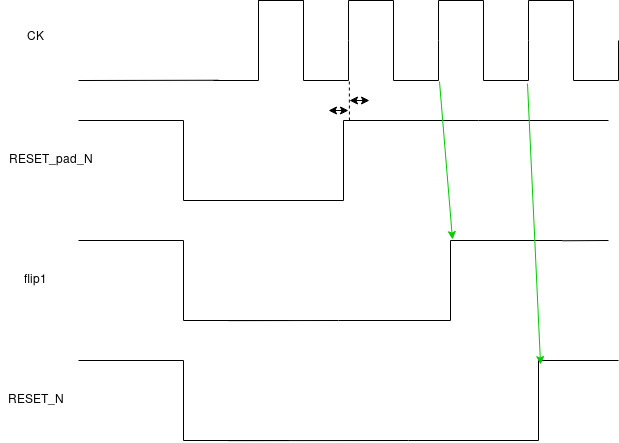
\includegraphics[height=0.34\linewidth,width=0.77\linewidth]{images/async_reset_chrono.png}
		\captionof{figure}{Waveform of a asynchronous reset synchronizer}
		\label{fig:async_synchronizer_chrono}
	\end{figure}

	\newpage
	\subsection*{Is there any reset synchronizer ? Code a reset synchronizer for asynchronous reset and add it to the
		design.}

	There was no synchronizer in the design at first, here is our implementation :

	\begin{figure}[h!]
		\centering
		\lstinputlisting[language=Vhdl, linerange={5739-5752}]{../src/mips_32_1p_mul_div.vhd}
		\captionof{figure}{VHDL of the reset synchronizer in the RTL design.}
		\label{fig:async_synchronizer_mips32_code}
	\end{figure}





	\newpage
	\section{Reporting}
	%https://vlsicad.ucsd.edu/Publications/Conferences/124/c124.pdf
	%K. D. Boese, A. B. Kahng and S. Mantik, "On the Relevance of Wire Load Models", (.ps), (.pdf), (.ppt), Proc. ACM International Workshop on System-Level Interconnect Prediction, April 2001, pp. 91-98.

	%WLM descriptions
	%http://asic-soc.blogspot.com/2013/07/wire-load-models-for-synthesis.html
	%http://tech.tdzire.com/what-is-a-wire-load-model/
	%http://mantravlsi.blogspot.com/2014/08/wire-load-model-wlm_1.html

	%https://www.edaboard.com/showthread.php?33505-Difference-between-quot-top-quot-amp-quot-enclosed-quot
	\subsection*{What is the area of the design ? How many cells are used ?}

	\par "Area of the design" definition : It is the sum of all the gates area plus the total net area. During synthesis there is no net area. 
	%calcule et precision area taille exact
	%https://community.cadence.com/cadence_technology_forums/f/logic-design/25863/what-does-area-reported-by-rtl-compiler-mean

	\par The Total Area can be found in the report table below, you can also see the number of cells :

	\begin{tabular}{|l|l|l|l|l|l|}
		\hline
		Instance                                  & Cells & Cell Area & Net Area & Total Area & Wireload  \\ \hline
		MIPS\_32\_1P\_MUL\_DIV                    & 14058 & 221458    & 0        & 221458   & area\_216Kto240K (S)  \\ \hline
	\end{tabular}

	\par(S) = wireload was automatically selected

	\subsection*{Which type of wireload model is used ? Why ?}
	The wireload model is specified as :   "Wireload mode : enclosed" by the command report area. We can see down the table that this WLM was chosen by default.

	\subsection*{What are the other types ? What wireload model are used for each hierarchy ? Why ?}

	\par According to the article On the Relevance of Wire Load Models\cite{WLM} the flow of creation of a chip can be divided into (All the quotations will come from this article in the next paragraph).:
	\begin{itemize}
		\item The front end  : from "RTL description and moves  through logic synthesis and optimization"
		\item The back end : "placement, routing, extraction and performance analysis" 
	\end{itemize}

	Before P\&R our design net parasitics and delays are unknown. We currently only know the fanout of the net in the block that the net belongs to. Therefore, in order to estimate the total length and capacitance of the net, WLM keep statistics of previously routed chips inside lookup tables.

	\par There are 3 types of wire-load models\footnote{\url{https://www.edaboard.com/showthread.php?33505-Difference-between-quot-top-quot-amp-quot-enclosed-quot}} :

	\begin{itemize}
		\item Top : All nets in the hierarchy will inherit the same wireload mode as the top-level block.
		\item Enclosed : All nets will inherit the WLM of the block that completely encloses the net even if it goes through sub-blocks.
		\item Segmented : If the net goes across several WLM, it will use the corresponding WLM on every portion of the net enclosed by a block.
	\end{itemize}

	\par Graphically\footnote{\url{http://asic-soc.blogspot.com/2013/07/wire-load-models-for-synthesis.html}} :

	\begin{figure}[h!]
		\centering
		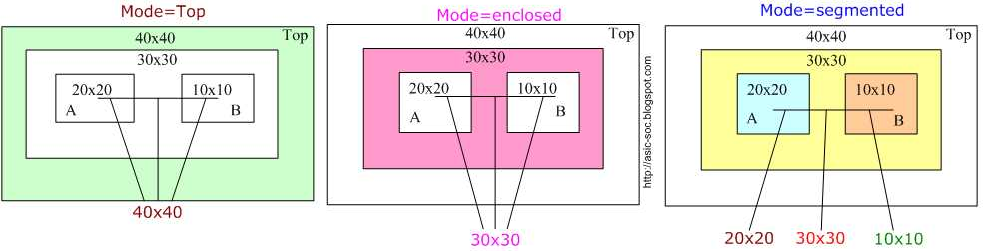
\includegraphics[width=\linewidth]{images/WLM.jpg}
		\captionof{figure}{Graphic modelization of the wire with different type of WLM, true value is at the bottom. We can see the different blocks colored
		}
		\label{fig:WLM}
	\end{figure}

	\newpage
	%http://www.siue.edu/~gengel/ece484LabMaterial/LogicSynthesisTutorial.pdf
	\subsection*{ \texttt{report timing} print the timing on the longest path. Examine the path (start point / end point etc.) and explain it.}
	\begin{itemize}
		\item Start-point  : I\_RI\_reg[31]/CP
		\item End-point    : NEXTPC\_RD\_reg[30]/D
	\end{itemize} 


	\begin{figure}[h!]
		\centering
		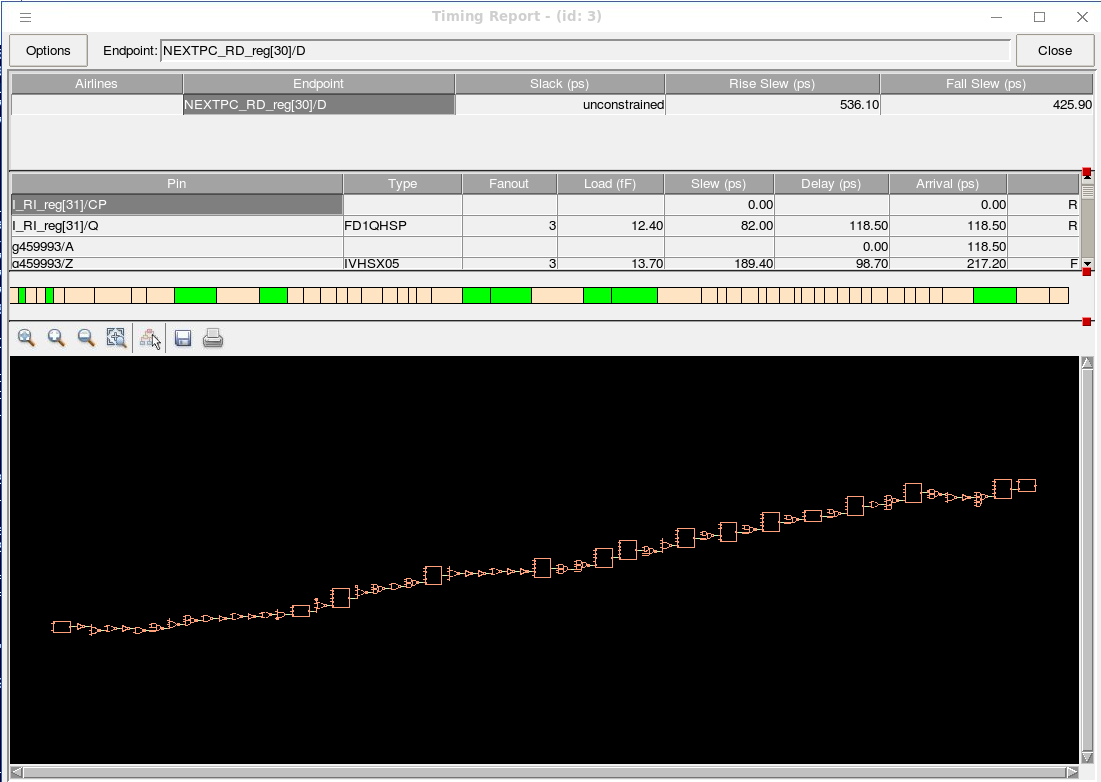
\includegraphics[width=\linewidth]{images/longestpath.png}
		\captionof{figure}{It is the longest path because 
		}
		\label{fig:WLM}
	\end{figure}

	We can see a report and the path from the selected flip-flop to the farthest flip-flop and all the cells between. The delay for each cell of the path is reported.

	\subsection*{What is the timing of the path ? What is the supposed max frequency the design is able to run ? }

	The timing of the path is visible at the last line :
	\begin{lstlisting}
		NEXTPC_RD_reg[30]/CP   setup                   0  +310   13992 R 
	\end{lstlisting}
	It is the sum of all delay in picoseconds to go through all the logic from the reg at the start-point to the reg at the endpoint. The max frequency will be the inverse of this longest path delay.

	\subsection*{You can see at the end of the report the following comment: \texttt{Timing slack : UNCONSTRAINED} What is a 'timing slack' ? Why it is 'UNCONSTRAINED' ?}

	As we can see in this course\footnote{\url{http://www.siue.edu/~gengel/ece484LabMaterial/LogicSynthesisTutorial.pdf}} the \texttt{report - timing - worst Path} will allow us to see the slowest path. We can see the value Slack on the graph above. but there is no value because we didn't constraint our design. This value will be positive in picoseconds if we have spare time. This implies the clock frequency can be increased. If it is a negative slack the design is failing. It is currently unconstrained because we didn't put any constraints.

	\subsection*{In order to check if the design is correctly constrained run: \texttt{report timing -lint} This command categorized the errors in 3 types, explain those types.}

	\begin{figure}[h!]
		\centering
		\begin{lstlisting}
			Lint summary
			Unconnected/logic driven clocks                                  0
			Sequential data pins driven by a clock signal                    0
			Sequential clock pins without clock waveform                  2877
			Sequential clock pins with multiple clock waveforms              0
			Generated clocks without clock waveform                          0
			Generated clocks with incompatible options                       0
			Generated clocks with multi-master clock                         0
			Paths constrained with different clocks                          0
			Loop-breaking cells for combinational feedback                   0
			Nets with multiple drivers                                       0
			Timing exceptions with no effect                                 0
			Suspicious multi_cycle exceptions                                0
			Pins/ports with conflicting case constants                       0
			Inputs without clocked external delays                          88
			Outputs without clocked external delays                        116
			Inputs without external driver/transition                       88
			Outputs without external load                                  116
			Exceptions with invalid timing start-/endpoints                  0

			Total:       3285
		\end{lstlisting}
		\captionof{figure}{\texttt{report -lint} output, as we can see there are more than 3 categories of errors.}
		\label{fig:report_lint}
	\end{figure}

	\begin{itemize}
		\item Sequential clock pins without clock waveform : pin not driven.
		\item Inputs without clocked external delays :  we need to use set\_input\_delay.
		\item Outputs without clocked external delays : we need to use set\_output\_delay.
		\item Inputs without external driver/transition : we need to set input ports transition slew rates.
		\item Outputs without external load : The delay is  a function between external load capacitance and input gate capacitance. thus it needs to be set.\footnote{\url{http://www.cse.psu.edu/~kxc104/class/cmpen411/14f/lec/C411L10InvDynamic.pdf, p12}}
	\end{itemize}











	\newpage
	\section{Constraints}
	\subsection{Reg-To-Reg}
	%https://sudip.ece.ubc.ca/rtl-compiler/
	\subsubsection*{Add in the RTLC script the command: \texttt{read\_sdc mips.sdc}}

	We have three main constraints  :

	\begin{figure}[h!]
		\centering
		\lstinputlisting[language=TXT, linerange={1-3}]{../src/constraints.sdc}
		\captionof{figure}{The three main constraints to set}
		\label{fig:main_constraints}
	\end{figure}

	\subsubsection*{Is the report timing -lint better ? Redo the synthesis with the new constraints and report the timing.}

	The \texttt{report timing -lint} is better :
	\begin{itemize}
		\item Errors about sequential clock pins without clock waveform has decreased from 2877 to 0.
		\item Errors about inputs/outputs without clocked external delays has decreased from 88/116 to 0/0.
		\item Inputs without external driver/transition has decreased from 88 to 87.
	\end{itemize}

	\subsubsection*{Why does the report show the clock now ?}
	That is because we applied constraints on : 
	\begin{itemize}
		\item input delay
		\item reg-to-reg delay
		\item output delay
	\end{itemize}

	The remaining error reports are due to input and output which are not connected.

	\begin{figure}[h!]
		\centering
		\lstinputlisting[language=TXT,linerange={182-190}]{../src/RS_design_constraint/step8_reporting.txt}
		\captionof{figure}{Report timing : Timing not met after STA with WLM}
		\label{fig:timing_not_met}
	\end{figure}

	\subsubsection*{What is the worst path ? What is the timing ? Is the slack positive ?}

	We have a timing violation on our new worst path :
	\begin{itemize}
		\item Start -point   : I\_RI\_reg [30]/ CP9
		\item End -point     : I\_A [14]
	\end{itemize}

	We can either optimize RTL or relax the clock or both. Nevertheless, if we relax the clock to resolve this worst path, all the timings in the design will be met.
	Currently, the worst path returns a timing negative slack, which value is -611ps, which is a reg-to-output path. In order to relax the clock perio,d we can take this value into account. At the moment there is no clock skew.

	\subsubsection*{Report the 10 worst paths.}

	The command is : \testtt{rc:/\textgreater report timing -worst 10}

	\begin{figure}[h!]
		\centering
		\begin{tabular}{lll}
			\hline
			\multicolumn{1}{|l|}{Timing slack (ps)} & \multicolumn{1}{l|}{Start-point}           & \multicolumn{1}{l|}{End-point}    \\ \hline
			\multicolumn{1}{|l|}{-611}              & \multicolumn{1}{l|}{I\_RI\_reg{[}30{]}/CP} & \multicolumn{1}{l|}{I\_A{[}14{]}} \\ \hline
			\multicolumn{1}{|l|}{-611}              & \multicolumn{1}{l|}{I\_RI\_reg{[}30{]}/CP} & \multicolumn{1}{l|}{I\_A{[}17{]}} \\ \hline
			\multicolumn{1}{|l|}{-611}              & \multicolumn{1}{l|}{I\_RI\_reg{[}30{]}/CP} & \multicolumn{1}{l|}{I\_A{[}14{]}} \\ \hline
			\multicolumn{1}{|l|}{-611}              & \multicolumn{1}{l|}{I\_RI\_reg{[}27{]}/CP} & \multicolumn{1}{l|}{I\_A{[}14{]}} \\ \hline
			\multicolumn{1}{|l|}{-611}              & \multicolumn{1}{l|}{I\_RI\_reg{[}30{]}/CP} & \multicolumn{1}{l|}{I\_A{[}17{]}} \\ \hline
			\multicolumn{1}{|l|}{-611}              & \multicolumn{1}{l|}{I\_RI\_reg{[}27{]}/CP} & \multicolumn{1}{l|}{I\_A{[}17{]}} \\ \hline
			\multicolumn{1}{|l|}{-611}              & \multicolumn{1}{l|}{I\_RI\_reg{[}30{]}/CP} & \multicolumn{1}{l|}{I\_A{[}14{]}} \\ \hline
			\multicolumn{1}{|l|}{-611}              & \multicolumn{1}{l|}{I\_RI\_reg{[}30{]}/CP} & \multicolumn{1}{l|}{I\_A{[}14{]}} \\ \hline
			\multicolumn{1}{|l|}{-611}              & \multicolumn{1}{l|}{I\_RI\_reg{[}27{]}/CP} & \multicolumn{1}{l|}{I\_A{[}14{]}} \\ \hline
			\multicolumn{1}{|l|}{-610}              & \multicolumn{1}{l|}{I\_RI\_reg{[}30{]}/CP} & \multicolumn{1}{l|}{I\_A{[}14{]}} \\ \hline
		\end{tabular}
		\captionof{figure}{Report of the 10 worst path of the design}
		\label{fig:worst_path}
	\end{figure}

	\subsubsection*{What is a launch clock ? What is a capture clock ?}

	\begin{itemize}
		\item launch clock : It is an event, the moment where data is launched by a FF.
		\item capture clock : It is an event, the moment where data is captured by another FF.
	\end{itemize}

	Here a graph representing the launch and capture from berkley university courses\footnote{\url{https://inst.eecs.berkeley.edu/~ee290c/sp17/lectures/Lecture27.pdf}} :
	\begin{figure}[h!]
		\centering
		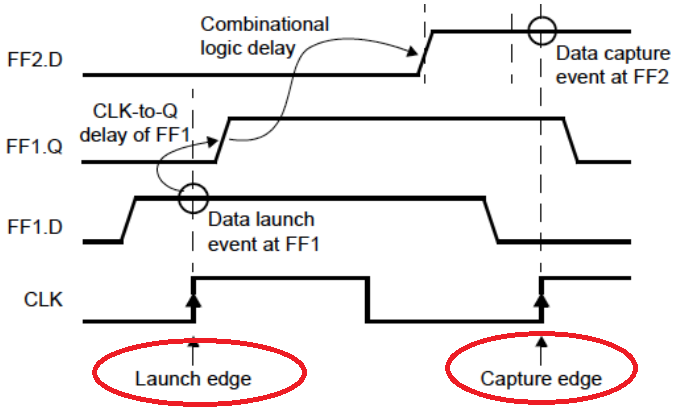
\includegraphics[width=0.55\linewidth]{images/launch_capture.png}
		\captionof{figure}{Example of Launch and capture clock represented from }
		\label{fig:launch_capture_graph}
	\end{figure}

	\begin{figure}[h!]
		\lstinputlisting[language=TXT,linerange={194-201}]{../src/RS_design_constraint/step8_reporting.txt}
		\captionof{figure}{Representation of the report from rtl compiler}
		\label{fig:launch_capture}
	\end{figure}

	\subsubsection*{Why did the tool choose this timing between the launch clock and the capture clock ?}

	Because it is the maximum time we have to capture the right data.

	\subsubsection*{What is the problem with your timing path in this case where the capture clock is another clock: CLOCK2 ? How would you solve the problem ? Hint: between two asynchronous clock domains the paths in between are usually not timed, hence, considered as false paths.}

	\begin{itemize}
		\item set\_false\_path command order to the compiler to ignore a path.
		\item set\_multi\_cycle command order to the compiler to look the capture after some cycle of the launch clock. 
	\end{itemize}

	It depends if the clocks are in a phase relationship. If yes, we use the set\_multicycle\_path command to fix it.
	If no, the slack between the launch and the capture clock is variable. So it's a clock domain crossing problem. The design must be ready for it, and we set this path with set\_false\_path command.

	"If two sequential elements are triggered by two different clocks then a common least common  multiple (LCM) of these two different clock periods should be considered to find the launch edge and capture edge for setup and hold timing" analysis\footnote{\url{http://www.idc-online.com/technical_references/pdfs/electronic_engineering/Fundamentals_of_Timing.pdf}}


	\subsubsection*{If a CLOCK2 would come from a clock divider which will generate CLOCK2 from
		CLOCK, therefore CLOCK2 is generated from CLOCK: what is the corresponding SDC command ?}
	We use the multi\_cycle\_path command.

	\newpage
	\subsubsection*{What is your worst path ? Is the timing met ?}
	There is only one clock domain, there might be a mistake in the questions.

	Still the timing is not met. In order to meet the timing we have to lower the frequency of the clock. We tried this :
	\begin{figure}[h!]
		\centering
		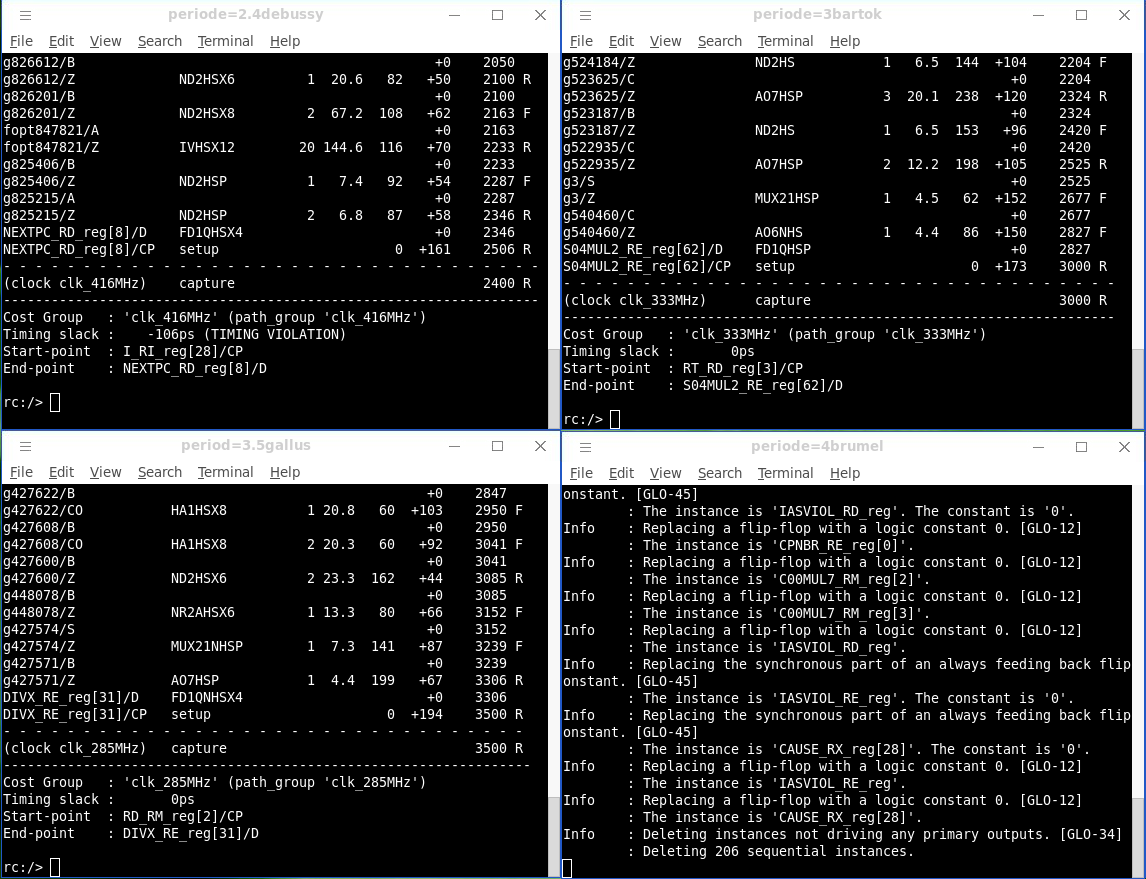
\includegraphics[width=\linewidth]{images/script.png}
		\captionof{figure}{Multiple synthesis at the same time period = 3ns wins. Timing slack is now 0.}
		\label{fig:scripting_synthesis}
	\end{figure}

	The problem is when you try \testtt{report summary} there is a fanout problem from DRC rule check :

	\begin{figure}[h!]
		\centering
		\begin{lstlisting}
			...
			Max_fanout design rule (violation total = 3.000)
			...
		\end{lstlisting}
	\end{figure}

	We don't have this problem if we set the periode to 3.5ns.


	\begin{figure}[h!]
		\centering
		\begin{lstlisting}
			Design Rule Check
			-----------------
			Max_transition design rule: no violations.

			Max_capacitance design rule: no violations.

			Max_fanout design rule: no violations.
		\end{lstlisting}
	\end{figure}

	It is overkill to do that because it can be resolved after and we can increase the fanout. Still, we want a robust design and it's our first full synthesis process so let's play safe with those values. We can still keep in mind that :
	\begin{figure}[h!]
		\centering
		\begin{lstlisting}
			Cost Group   : 'clk_392MHz' (path_group 'clk_392MHz')
			Timing slack :       0ps 
			Start-point  : I_RI_reg[28]/CP
			End-point    : NEXTPC_RD_reg[6]/D
		\end{lstlisting}
	\end{figure}
	This is the best value to have no timing slack violation.

	%%%%%%%%%%%%%%%%%%%%%%%%%%%%%%%%%%%%%%%%%%%%%%%%%%%%%%%%%%%%%%%%%%
	\subsection{Input-to-Reg}

	\subsubsection*{Let's consider that the inputs in the clock domain CLOCK takes 1.2 nanosecond to come. Even before running the tool can you already know if the timing will be met ? Explain (drawing + maths).}

	The clock period must be greater than the worst path additionned with the input delay. We have a majoration of Xns for the period in order to have a design that synthetize without any timing negative slack.
	\begin{gather}
		WPT = 2311 ps\\
		WPT\_minimal_majoration = 2550 ps\\
		WPT\_maximal_majoration = 3500ps\\
		I/O\_delay = 1200 ps\\
		clock\_period > worst\_path\_timing + I/O\_delay\\
		clock\_period > (2311+1200) = 3511 ps\\
		freq = 1 / 0.003511 < freq = 1 / 0.0036 \\
		freq >= 276mhz\\
	\end{gather}

	We tried 2.4ns, 3.5ns and 4.7ns. As we could predict 2.4ns does not work at all but here are the results for 3.5 and 4.7 :

	\begin{figure}[h!]
		\centering
		\begin{lstlisting}
			Cost Group   : 'clk_285MHz' (path_group 'clk_285MHz')
			Timing slack :       0ps 
			Start-point  : I_RI_reg[31]/CP
			End-point    : NEXTPC_RD_reg[26]/D


			Cost Group   : 'clk_212MHz' (path_group 'clk_212MHz')
			Timing slack :       0ps 
			Start-point  : RD_RE_reg[0]/CP
			End-point    : DIVX_RE_reg[31]/D
		\end{lstlisting}

	\end{figure}

	\subsubsection*{Please write the corresponding SDC command and report the timing. Is the result match your expectation ? As it is an unrealistic constraint at this frequency, let's consider the minimum input constraint.}
	\begin{figure}[h!]
		\centering
		\begin{lstlisting}
			create_clock -name clk_285MHz -period 3.5 [get_port CK]
			set_input_delay 1.2 -clock clk_285MHz [get_port RESET_N]
			set_input_delay 1.2 -clock clk_285MHz [get_port IT_N]
			set_input_delay 1.2 -clock clk_285MHz [get_port CPU_NBR]
			set_input_delay 1.2 -clock clk_285MHz [get_port I_RBERR]
			set_input_delay 1.2 -clock clk_285MHz [get_port I_ACCPT]
			set_input_delay 1.2 -clock clk_285MHz [get_port I_IN]
			set_input_delay 1.2 -clock clk_285MHz [get_port D_RBERR]
			set_input_delay 1.2 -clock clk_285MHz [get_port D_WBERR]
			set_input_delay 1.2 -clock clk_285MHz [get_port D_ACCPT]
			set_input_delay 1.2 -clock clk_285MHz [get_port D_IN]
			set_input_delay 1.2 -clock clk_285MHz [get_port MCHECK_N]
		\end{lstlisting}
		\captionof{figure}{input delay commands.}
		\label{fig:constraints_input}
	\end{figure}

	\newpage
	\subsubsection*{Open the library .lib file and find the CK-\textgreater Q timing (access time). Takes this value as input delay.}
	The flip-flop used here is the "FD1QHSP" cell in library. The the minimal edge timing of the output is equal to the best timing of a transition, it is 0.05438ns. The value of CK-\textgreater Q is 0.05438ns.


	\subsubsection*{Rerun the tool and report the new timing. What does it mean ? Is the timing met ? What is the timing slack ?}

	Here are the results for 392mhz and 285mhz clock :

	\begin{figure}[h!]
		\centering
		\begin{lstlisting}
			Cost Group   : 'clk_392MHz' (path_group 'clk_392MHz')
			Timing slack :       0ps 
			Start-point  : I_RI_reg[29]/CP
			End-point    : NEXTPC_RD_reg[16]/D

			Cost Group   : 'clk_285MHz' (path_group 'clk_285MHz')
			Timing slack :       0ps 
			Start-point  : RD_RM_reg[2]/CP
			End-point    : DIVX_RE_reg[31]/D
		\end{lstlisting}
	\end{figure}


	%----------------------------------------------------------------------------------
	%Indeed, when we target a clock of 3600ps we get a negative slack of -3ps for the same worst data-path! So the result %match pretty good with our expectation, but not exactly. More than, we added 109ps more what we must in theoretically.
	%And the optimization to get a timing met are at a medium effort, and in incremental mode. Incremental mode mean the engine try to optimize until to get a timing met. It's why we get a timing to 0ps for the worst path.


	%And we set all I/O delays with this value and the clock to 2400ps. They was a timing violation of -161ps. So we start a new synthesis with high effort :
	%{\colorbox{Gray!50}{\textcolor{RubineRed}{"synthesize -effort high -to\_mapped"}}}
	%After that, the timing is clean.
	%-----------------------------------------------------------------------------------

	%%%%%%%%%%%%%%%%%%%%%%%%%%%%%%%%%%%%%%%%%%%%%%%%%%%%%%%%%%%%%%%%%%
	\newpage
	\subsection{Reg-To-Output}

	\subsubsection*{First, let's consider an output delay on all outputs, synchronized to CLOCK. The output delay is 1.2ns. Please write the correct SDC command and report the timing.}

	\begin{figure}[h!]
		\centering
		\begin{lstlisting}
			create_clock -name clk_285MHz -period 2.55 [get_port CK]
			set_output_delay 1.2 -clock clk_392MHz [get_port I_A]
			set_output_delay 1.2 -clock clk_392MHz [get_port I_RQ]
			set_output_delay 1.2 -clock clk_392MHz [get_port MODE]
			set_output_delay 1.2 -clock clk_392MHz [get_port I_ACK]
			set_output_delay 1.2 -clock clk_392MHz [get_port I_BEREN]
			set_output_delay 1.2 -clock clk_392MHz [get_port I_INLINE]
			set_output_delay 1.2 -clock clk_392MHz [get_port D_A]
			set_output_delay 1.2 -clock clk_392MHz [get_port D_BYTSEL]
			set_output_delay 1.2 -clock clk_392MHz [get_port D_RQ]
			set_output_delay 1.2 -clock clk_392MHz [get_port D_RW]
			set_output_delay 1.2 -clock clk_392MHz [get_port D_SYNC]
			set_output_delay 1.2 -clock clk_392MHz [get_port D_REG]
			set_output_delay 1.2 -clock clk_392MHz [get_port D_LINKED]
			set_output_delay 1.2 -clock clk_392MHz [get_port D_RSTLKD]
			set_output_delay 1.2 -clock clk_392MHz [get_port D_CACHE]
			set_output_delay 1.2 -clock clk_392MHz [get_port D_CACHOP]
			set_output_delay 1.2 -clock clk_392MHz [get_port D_OUT]
			set_output_delay 1.2 -clock clk_392MHz [get_port D_ACK]
			set_output_delay 1.2 -clock clk_392MHz [get_port SCOUT]
		\end{lstlisting}
		\captionof{figure}{output delay commands}
		\label{fig:constraints_output}
	\end{figure}

	\subsubsection*{Is the timing met ? What is the timing slack ?}

	Here are the results for 285mhz and 212mhz clock :
	\begin{figure}[h!]
		\centering
		\begin{lstlisting}
			Cost Group   : 'clk_285MHz' (path_group 'clk_285MHz')
			Timing slack :     -85ps (TIMING VIOLATION)
			Start-point  : I_RI_reg[28]/CP
			End-point    : I_A[28]


			Cost Group   : 'clk_212MHz' (path_group 'clk_212MHz')
			Timing slack :       1ps 
			Start-point  : RD_RE_reg[3]/CP
			End-point    : DIVX_RE_reg[30]/D
		\end{lstlisting}
	\end{figure}

	\subsubsection*{What is the worst path ? Why is it so long ?}

	\subsubsection*{Is the timing met now ?}

	Timing is met for values : 392mhz and 0.05438ns of output delay (it was only for test).
	We started a synthesis with high effort :
	{\colorbox{Gray!50}{\textcolor{RubineRed}{synthesize -effort high -to\_mapped}}}

	\begin{figure}[h!]
		\centering
		\begin{lstlisting}
			Cost Group   : 'clk_392MHz' (path_group 'clk_392MHz')
			Timing slack :       0ps 
			Start-point  : I_RI_reg[28]/CP
			End-point    : I_TYPE_RD_reg[7]/D
		\end{lstlisting}
	\end{figure}

	%%%%%%%%%%%%%%%%%%%%%%%%%%%%%%%%%%%%%%%%%%%%%%%%%%%%%%%%%%%%%%%%%%
	\newpage
	\section{Report timing}
	\subsection{Through}
	\subsubsection{
		Print the timing path through the output Q of a flip-flop of your choice. Draw the path and explain it.}
	We selected this flip-flip from netlist :
	\begin{itemize}
		\item Instance : I\_TYPE\_RM\_reg[11]
		\item libcell: FD1QHSP
	\end{itemize}

	And we run the next command : {\colorbox{Gray!50}{\textcolor{RubineRed}{report timing -through I\_TYPE\_RM\_reg[11]}}}

	Return :

	-- Timing slack :       6ps\\
	-- Start-point  : I\_TYPE\_RM\_reg[11]/CP\\
	-- End-point    : DIVY  \_RE\_reg[26]/D\\

	The instance is a flip-flop, this command in this case, is equal to a "report timing -from".
	So we use the same command on a cell of this path which is not a flip-flop to explain report-through result: 
	{\colorbox{Gray!50}{\textcolor{RubineRed}{report timing -through g1300010}}}\\
	And we get the same result :\\
	-- Timing slack :       6ps\\
	-- Start-point  : I\_TYPE\_RM\_reg[11]/CP\\
	-- End-point    : DIVY  \_RE\_reg[26]/D\\

	In order to see this netlist path, we report the timing from start-point on gui :
	\begin{figure}[h!]
		%\centering
		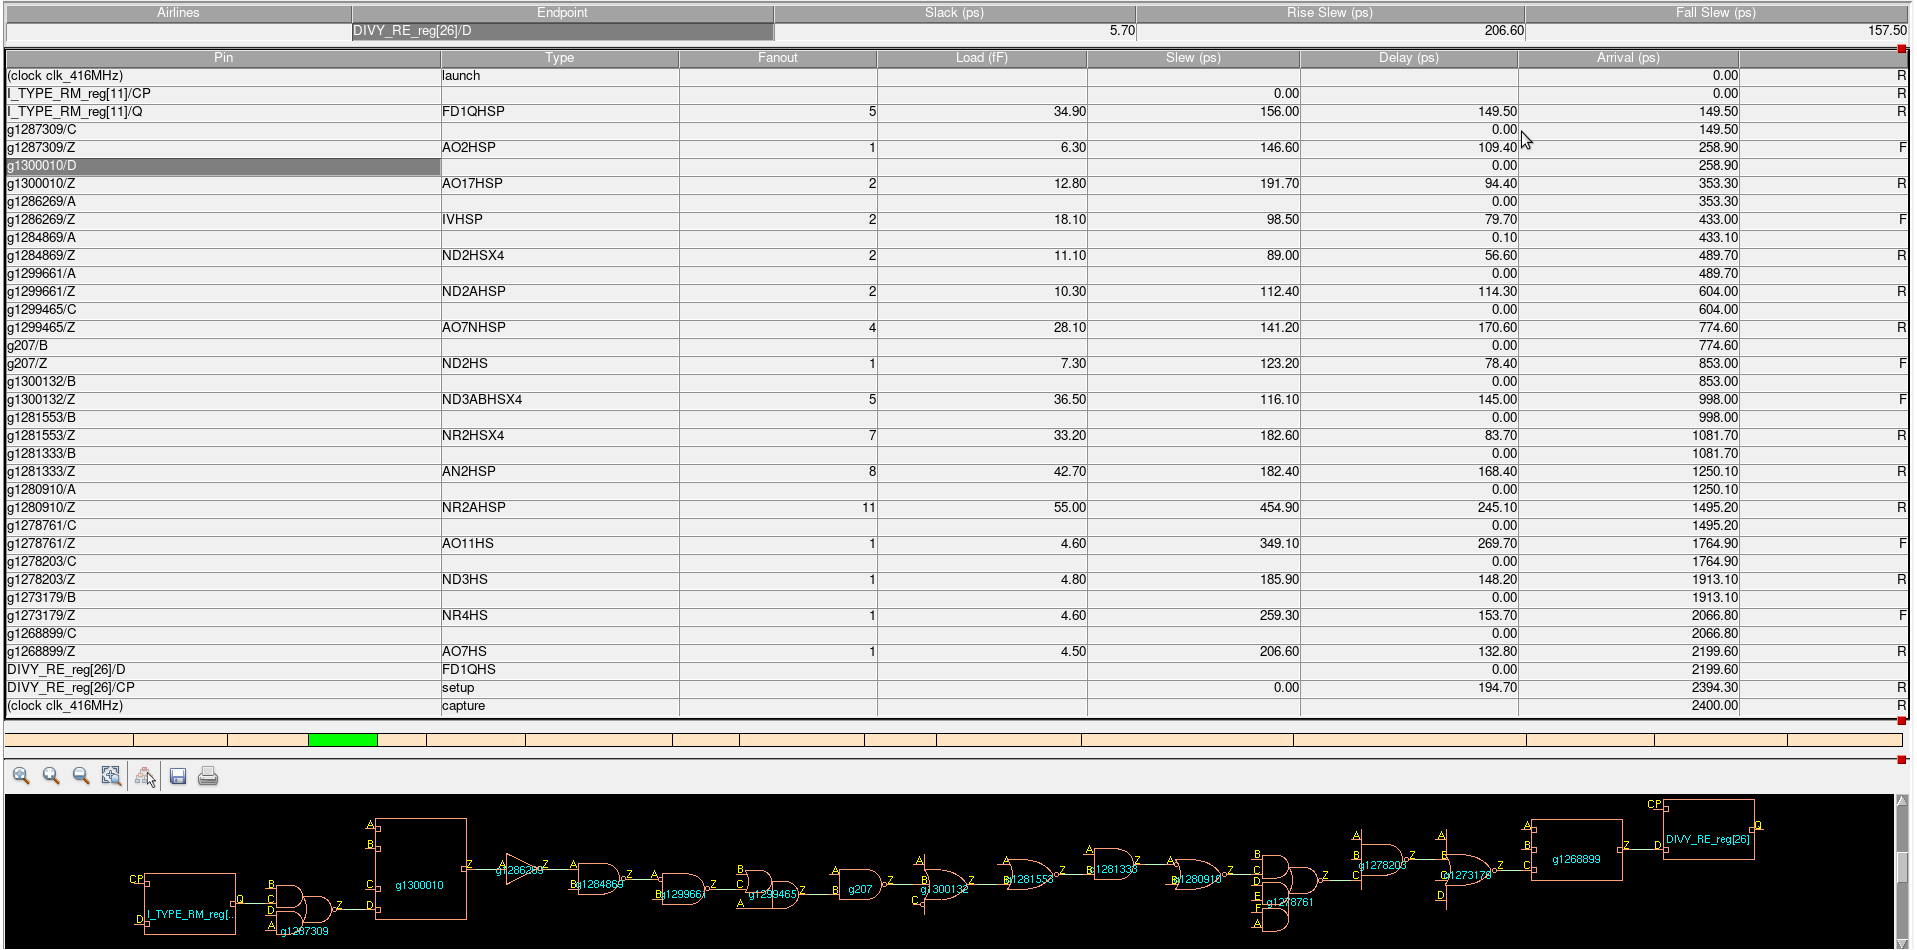
\includegraphics[width=1.1\linewidth, frame]{images/through_report.png}
		\captionof{figure}{Resume of a reg-to-reg path with all cells delays.}
		\label{fig:through_report_draw}
	\end{figure}

	\subsection{From}


	Command : {\colorbox{Gray!50}{\textcolor{RubineRed}{report timing -from I\_TYPE\_RM\_reg[11]}}}\\

	Results :\\
	-- Timing slack :       6ps \\
	-- Start-point  : I\_TYPE\_RM\_reg[11]/CP\\
	-- End-point    : DIVY\_RE\_reg[26]/D\\

	\subsection{To}

	Command : {\colorbox{Gray!50}{\textcolor{RubineRed}{report timing -to I\_TYPE\_R\_reg[11]}}}\\

	Results :\\
	-- Timing slack :     12ps \\
	-- Start-point  : DRQ\_RE\_reg/CP\\
	-- End-point    : I\_TYPE\_RM\_reg[11]/D\\

	\subsection{From-To}

	Command : {\colorbox{Gray!50}{\textcolor{RubineRed}{report timing -from I\_TYPE\_RM\_reg[11] -to DIVY\_RE\_reg[26]/D}}}\\

	Results :\\
	-- Timing slack :       6ps\\ 
	-- Start-point  : I\_TYPE\_RM\_reg[11]/CP\\
	-- End-point    : DIVY\_RE\_reg[26]/D\\


	%%%%%%%%%%%%%%%%%%%%%%%%%%%%%%%%%%%%%%%%%%%%%%%%%%%%%%%%%%%%%%%%%%
	\newpage
	\section{Optimizations}
	By default the tool will optimize only the worst negative slack (WNS). WNS optimization produces better area, but more violations. You can tell the synthesizer to optimize the total negative slack (TNS). The TNS approach produces fewer violations, meaning fewer issues in the place-and-route stage, but on the other hand runtime will increase. As a general rule, always turn on TNS optimization.

	\texttt{set\_attribute endpoint\_slack\_opto true}

	result :
	\begin{figure}[h!]
		\centering
		\begin{lstlisting}
			WITHOUT HIGH EFFORT
			Cost Group   : 'clk_392MHz' (path_group 'clk_392MHz')
			Timing slack :     -18ps (TIMING VIOLATION)
			Start-point  : I_RI_reg[26]/CP
			End-point    : NEXTPC_RD_reg[30]/D

			WITH HIGH EFFORT
			Cost Group   : 'clk_392MHz' (path_group 'clk_392MHz')
			Timing slack :       0ps 
			Start-point  : I_RI_reg[30]/CP
			End-point    : I_TYPE_RD_reg[23]/D
		\end{lstlisting}
	\end{figure}


	\subsection*{Explain the difference between WNS and TNS.}

	%Setup
	That are slack for setup timing :
	\begin{itemize}
		\item WNS = Worst Negative Slack = the worst of all negative slack
		\item TNS = Total Negative Slack = sum of the negative slack paths
	\end{itemize}
	The TNS with WNS, lets appreciate the number of negative slack path.

	%Hold
	NB : For hold timing violation after clock-tree, we look the WHS(=WNS) and the THS(=TNS).

	%Width
	%WPWS : Worst Pulse Width Slack
	%TPWS : Total Pulse Width Slack



	%%%%%%%%%%%%%%%%%%%%%%%%%%%%%%%%%%%%%%%%%%%%%%%%%%%%%%%%%%%%%%%%%%
	\newpage
	\section{Design for Test : DFT}

	After fabrication of IC, many defects can appear. There can be numerous failures and, found those is like looking for a needle in a haystack. Then, we use the DFT to do it. 
	DFT boils down to an abstraction of a set defects to a faulty model.
	An example is a short-circuit between a gate and power supply, results in a signal "stuck" to a static state. So, detection of a specific abstract fault reveals a defect into a specific set of defects.
	This abstraction of defect makes their detection easier.

	In summary, the DFT allows to detect fabrication errors.
	There are many models, like static stuck-at-fault model like above, or the same in a dynamic model (dynamic is a superset of static) to detect bad connection.

	In fact, that resume to add "shadow" logic into the design. The DFT methods must be integrated in design conception step.

	%functional pattern != structural test
	\subsection*{The insertion of the scan-chains are done during the synthesis. Explain what is a scan-chain and the purpose of it ?}

	A scan-test is the use of a sequential circuit. It resumed the ATPG to a combinational test problem, which is easier to solve. The scan-test making all flip-flop scannable, by chain them. That allows to put a value in each flip-flop at a time, and to get them at another time. To compare an expected value with a real value to detect a fault. And allow to automate the test by using test-pattern.

	\subsection*{Insert 4 scan-chains using functionnal pins for scan-ins and scan-outs.}

	\begin{figure}[h!]
		\centering
		\lstinputlisting[language=bash, linerange={387-405}]{src/CMD.txt}
		\captionof{figure}{Mains command to add a scan-chain into the design}
		\label{fig:scan-chain commands}
	\end{figure}

	\subsection*{For timing constraints, are you using the same sdc file as the functional mode ? Why not ?}

	No, we use a slow clock for the scan-chain and add the port : TDI, TDO, scan\_en, test\_mode. And we select the same I/O delay.

	\subsection*{Write the corresponding .sdc for the test mode as well as update the .sdc for the functional mode.}

	\begin{figure}[h!]
		\centering
		\lstinputlisting[language=bash, linerange={80-90}]{src/constraints.sdc}
		\captionof{figure}{Few constrains for test}
		\label{fig:scan-chain constraints}
	\end{figure}


	%%%%%%%%%%%%%%%%%%%%%%%%%%%%%%%%%%%%%%%%%%%%%%%%%%%%%%%%%%%%%%%%%%
	\section{Writing outputs}
	\subsection*{Open the generated netlist and check if everything seems ok. Open up the generated sdc and compare it to the input one. What are the differences ? What is a “set\_dont\_use” ? Why the tool should not use some cells ?}
	We can see as different :
	The precision about the wireloadmodel, set of capacitance unit and clock unit, setclockgating, some setdontuse (the \texttt{set\_dont\_use} command is used to exclude cells from the target library. Design Compiler does not use these excluded cells during optimization.)

	%%%%%%%%%%%%%%%%%%%%%%%%%%%%%%%%%%%%%%%%%%%%%%%%%%%%%%%%%%%%%%%%%%
	\section{Equivalence checking}
	\subsection*{RTLC is able to generate the script to automatically run LEC (Conformal), what is an equivalence checking tool ? why do we need to run such a tool ? why do not use simulation ?}
	Equivalence checking is the formal verification of a design, it uses boolean logic to verify the veracity of a design or if the design is equivalent after operations on it, for example optimisation. It is necessary to verify that even after that optimisation phase the function is still the same. It is impossible to prove a circuit without equivalence checking, there are too many cases for human lifetime of testing.

	\subsection*{Run LEC and check that your netlist is equivalent to the original RTL.}
	LEC does not work.

	\newpage
	\chapter{SoC Encounter}
	\section{Environment}
	\section{Design import}
	\subsection*{The netlists}
	\subsection*{The physical Libraries}
	\subsubsection*{For Technology/Physical Libraries, select LEF files and fill in the correct LEF files. What is a LEF file ?}
	Layer Exchange Format : Its a lite physical library for abstract model different from library used to GDSII
	\subsection*{Global Nets : Power Nets}
	\subsubsection*{For the Power section, enter the name of the power nets. For “Power Nets” enter, let's say
		“vdd\_core” and for “Ground Nets” “gnd\_core”. Why do we have to enter this power net information ?}

	Because those are the future global connection of VDD and GND for the whole die. It will be used for the ring/stripes.

	\subsection*{IO assignment file}
	\subsubsection*{What is an IO assignment file ?}
	IO Assignement File : It is an optional file that is used to instruct the tool where to place IO pins. Without any file the tool will determine these locations automatically. \footnote{\url{https://community.cadence.com/cadence_technology_forums/f/digital-implementation/1378/design-io-assignment-file-generation}}

	\subsection*{Check Design}
	\subsubsection*{Check the standard cell number, the area, the number of instances, the number of primary
		inputs/outputs. Is it ok ?}

	Currently everything is OK !

	\begin{lstlisting}
		rc:/> report summary
		...
		Instance       Cells  Cell Area  Net Area  Total Area     Wireload        
		-------------------------------------------------------------------------------
		MIPS_32_1P_MUL_DIV  14439     225299         0      225299 area_216Kto240K (S) 

		encounter 1> checkDesign -netlist
		############################################################################
		# Encounter Netlist Design Rule Check
		# Sun Feb 23 16:02:31 2020
		############################################################################
		Design: MIPS_32_1P_MUL_DIV

		------ Design Summary:
		Total Standard Cell Number   (cells) : 14439
		Total Block Cell Number      (cells) : 0
		Total I/O Pad Cell Number    (cells) : 0
		Total Standard Cell Area     ( um^2) : 225299.05
	\end{lstlisting}




	\subsubsection*{Are there multi-driver nets ? What is that ? Is it a problem ?}
	There is no multi-driver nets :\footnote{\url{https://wiki.nus.edu.sg/display/EE2020DP/\%5BDRC+23-20\%5D+Rule+violation+\%28MDRV-1\%29+Multiple+Driver+Nets}}
	\begin{lstlisting}
		encounter 1> checkDesign -netlist
		...
		Number of nets with multiple drivers           : 0

		##############################
		example of multi-driver net :
		always @ (posedge CLK)
		y = y + 1;

		always @ (posedge CLK2)
		y = y + 3;
	\end{lstlisting}


	\subsubsection*{Now check that the SDC is correctly read, run: \texttt{report\_clocks Is it ok ?}
		Explain L-\textgreater L, L-\textgreater LT, T-\textgreater LL and T-\textgreater LT.}
	Everything is still ok.
	\begin{itemize}
		\item L-\textgreater L : we didn't find that.
		\item L-\textgreater LT : we didn't find that.
		\item T-\textgreater LL : we didn't find that.
		\item T-\textgreater LT : we didn't find that.
	\end{itemize}
	\begin{lstlisting}
		encounter 2> report_clocks
		+-------------------------------------------------------------------------------+ 
		|                              Clock Descriptions                               | 
		|-------------------------------------------------------------------------------| 
		|            |        |       |        |       |       |       Attributes       | 
		|------------+--------+-------+--------+-------+-------+------------------------| 
		| Clock Name | Source |  View | Period |  Lead | Trail | Generated | Propagated | 
		|------------+--------+-------+--------+-------+-------+-----------+------------| 
		| clk_200MHz |   CK   | setup |  5.000 | 0.000 | 2.500 |     n     |     n      | 
		+-------------------------------------------------------------------------------+ 
	\end{lstlisting}

	\subsubsection*{Reload encounter with the new SDC and check with report\_clock that the new command is
		correctly understood. \texttt{set\_propagated\_clock [all\_clocks]}}

	We can see that the clock is now propagated in the section Propagated inside the section Attributes.

	\begin{lstlisting}
		encounter 1> report_clocks
		+-------------------------------------------------------------------------------+ 
		|                              Clock Descriptions                               | 
		|-------------------------------------------------------------------------------| 
		|            |        |       |        |       |       |       Attributes       | 
		|------------+--------+-------+--------+-------+-------+------------------------| 
		| Clock Name | Source |  View | Period |  Lead | Trail | Generated | Propagated | 
		|------------+--------+-------+--------+-------+-------+-----------+------------| 
		| clk_200MHz |   CK   | setup |  5.000 | 0.000 | 2.500 |     n     |     y      | 
		+-------------------------------------------------------------------------------+ 
	\end{lstlisting}

	\newpage
	\section{Floorplanning}

	\subsection*{You can see beside the label “Core Utilization” the classical number 0.7. This specifies the core
		area, here it means that 70\% of the design is filled with cells. You can play with this number to
		change the core area. This has an impact on the congestion of the design, in other words on the
		routability of the design. Explain why.}

	Our design needs to have some space on the floorplaning. The last 30\% will be used for IOpad, rings etc. It is the allocated space for our design.

	\section{Power Planning}
	\subsection*{Connecting to Global Nets}
	\subsubsection*{check if everything is correct ? No ? Please correct and rerun. Click “Close”. If you do not find the name of the power pins in the LEF try “vdd” and “gnd”.}
	Everything is OK.

	\subsection*{Add Rings}
	\subsubsection*{These layers are noted V, the first ones are noted H. Explain that :}
	The one noted V are for vertical and the one noted H are for horrizontal.

	\subsection*{Add Stripes, SRoute, Saving the floorplan}
	Everything is still OK.

	\begin{figure}[h!]
		\centering
		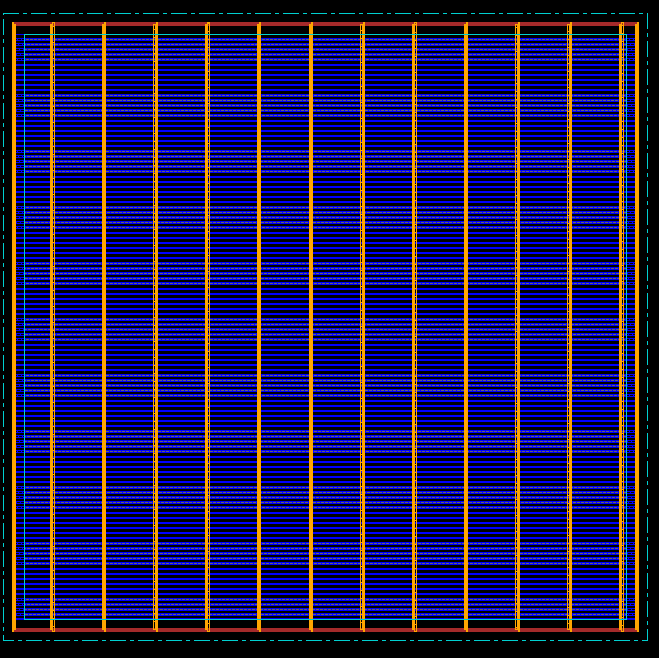
\includegraphics[width=0.50\linewidth, frame]{images/floorandpower_plan.png}
		\captionof{figure}{Result of the floor and power plan.}
		\label{fig:floor_power_plan}
	\end{figure}

	\newpage
	\section{Place Design}
	\subsubsection*{Standard Cells Placement}
	Result : 
	\begin{figure}[h!]
		\centering
		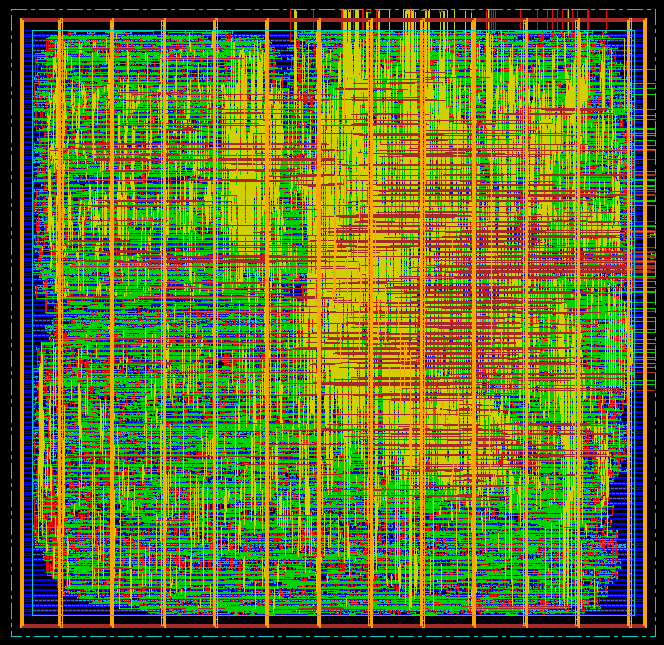
\includegraphics[width=\linewidth, frame]{images/place_std_cells.png}
		\captionof{figure}{Result of place standard cells.}
		\label{fig:place_std_cells}
	\end{figure}

	\newpage
	\section{Trial Route}
	We didn't find the diamonds. We have remarked that there is a problem about the size of a cell that is too big :
	\begin{lstlisting}
		**WARN: (ENCTR-3824):	The standard cell row height appears to be too large.
		Estimated standard cell row height = 20 metal3 tracks
	\end{lstlisting}

	Rest of the output is :

	\begin{lstlisting}
		encounter 2> *** Starting trialRoute (mem=822.8M) ***

		There are 0 guide points passed to trialRoute for fixed pins.
		There are 0 guide points passed to trialRoute for pinGroup/netGroup/pinGuide pins.
		Options:  -maxRouteLayer 6 -gcellSizeX 4 -gcellSizeY 2 -floorPlanMode -noPinGuide

		**WARN: (ENCTR-3824):	The standard cell row height appears to be too large.
		Estimated standard cell row height = 20 metal3 tracks

		Phase 1a-1d Overflow: 0.02% H + 1.54% V (0:00:00.1 812.5M)

		Phase 1e-1e Overflow: 0.00% H + 0.71% V (0:00:00.0 813.2M)

		Phase 1l Overflow: 0.02% H + 3.98% V (0:00:00.2 810.4M)


		Congestion distribution:

		Remain	cntH		cntV
		--------------------------------------
		-5:	0	 0.00%	48	 0.56%
		-4:	0	 0.00%	26	 0.30%
		-3:	0	 0.00%	28	 0.33%
		-2:	0	 0.00%	37	 0.43%
		-1:	2	 0.02%	65	 0.76%
		--------------------------------------
		0:	6	 0.07%	63	 0.74%
		1:	9	 0.11%	80	 0.93%
		2:	16	 0.19%	76	 0.89%
		3:	26	 0.30%	101	 1.18%
		4:	20	 0.23%	107	 1.25%
		5:	8489	99.08%	7937	92.64%


		Total length: 6.906e+05um, number of vias: 109396
		M1(H) length: 1.085e+04um, number of vias: 57458
		M2(V) length: 2.167e+05um, number of vias: 40991
		M3(H) length: 2.678e+05um, number of vias: 8296
		M4(V) length: 1.204e+05um, number of vias: 2522
		M5(H) length: 7.086e+04um, number of vias: 129
		M6(V) length: 4.019e+03um

		Peak Memory Usage was 818.7M 
		*** Finished trialRoute (cpu=0:00:01.0 mem=819.8M) ***
	\end{lstlisting}

	\newpage
	\section{Timing Analysis}
	\subsection*{Choose the correct “Design Stage” and explain your choice}
	We are currently Pre-CTS, just before the clock tree synthesis but after the place.

	\subsection*{Check if the the worst negative slack (WNS) is positive. Is the timing met ?}
	As we can see the timing is not met, WNS is negative.

	\begin{lstlisting}
		timeDesign Summary                             
		+--------------------+---------+---------+---------+---------+---------+---------+
		|     Setup mode     |   all   | reg2reg | in2reg  | reg2out | in2out  | clkgate |
		+--------------------+---------+---------+---------+---------+---------+---------+
		|           WNS (ns):| -24.406 | -24.406 | -24.126 |   N/A   |   N/A   |   N/A   |
		|           TNS (ns):|-25961.3 |-25961.3 |-25216.7 |   N/A   |   N/A   |   N/A   |
		|    Violating Paths:|  2148   |  2148   |  1770   |   N/A   |   N/A   |   N/A   |
		|          All Paths:|  6714   |  6697   |  1798   |   N/A   |   N/A   |   N/A   |
		+--------------------+---------+---------+---------+---------+---------+---------+
	\end{lstlisting}

	\subsection*{Optimize the design with the \texttt{optDesign} command. Redo a \texttt{timeDesign}. Is the timing met now ? What is the slack ?}
	Timing is met now, slack is positive.
	\begin{lstlisting}
		optDesign Final Summary                             
		+--------------------+---------+---------+---------+---------+---------+---------+
		|     Setup mode     |   all   | reg2reg | in2reg  | reg2out | in2out  | clkgate |
		+--------------------+---------+---------+---------+---------+---------+---------+
		|           WNS (ns):|  0.124  |  0.124  |  0.523  |   N/A   |   N/A   |   N/A   |
		|           TNS (ns):|  0.000  |  0.000  |  0.000  |   N/A   |   N/A   |   N/A   |
		|    Violating Paths:|    0    |    0    |    0    |   N/A   |   N/A   |   N/A   |
		|          All Paths:|  6714   |  6697   |  1798   |   N/A   |   N/A   |   N/A   |
		+--------------------+---------+---------+---------+---------+---------+---------+
	\end{lstlisting}

	\subsection*{Report the timing and check in the floorplan where is the path.}
	\begin{lstlisting}
		encounter 4> report_timing                 
		Path 1: MET Setup Check with Pin HI_RW_reg[29]/CP 
		Endpoint:   HI_RW_reg[29]/D     (^) checked with  leading edge of 'clk_200MHz'
		Beginpoint: S00MUL7_RM_reg[4]/Q (^) triggered by  leading edge of 'clk_200MHz'
	\end{lstlisting}

	\newpage
	\begin{figure}[h!]
		\centering
		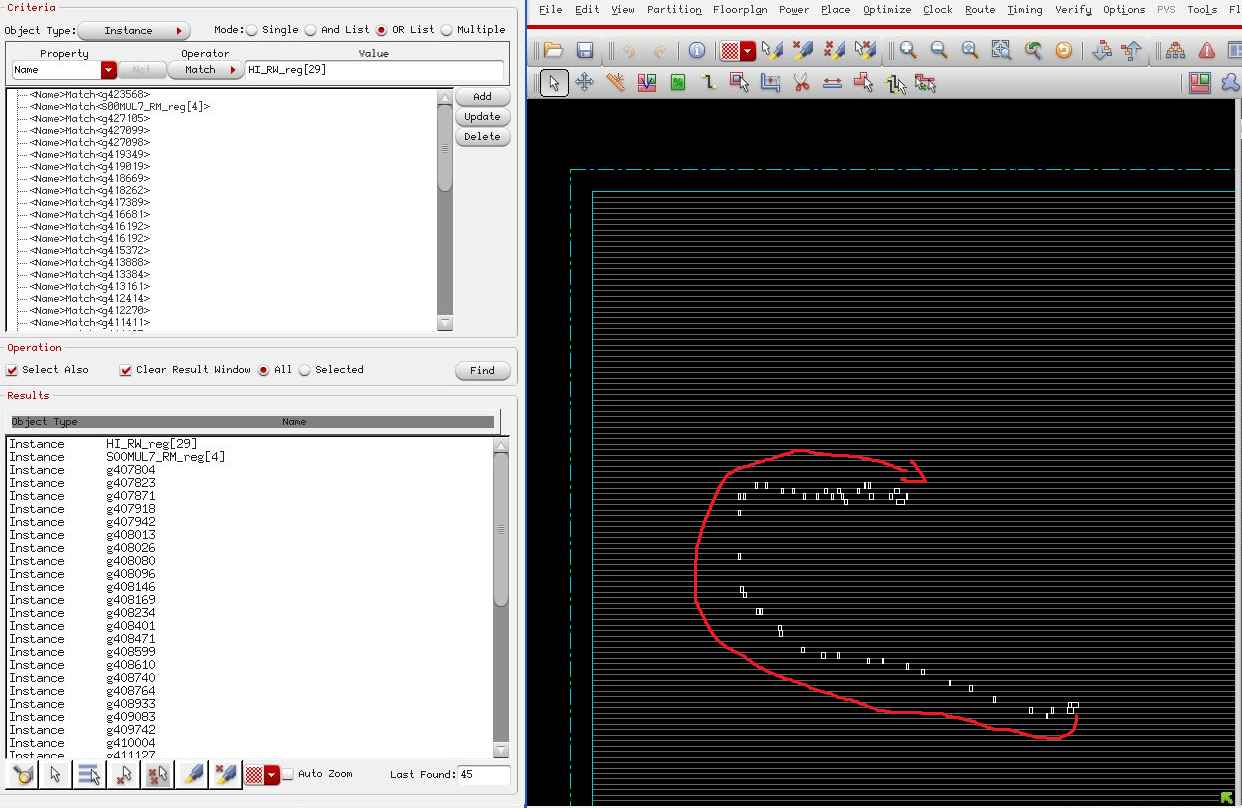
\includegraphics[width=\linewidth, frame]{images/pathtiminganalysis.png}
		\captionof{figure}{Longest path found between the two regs.}
		\label{fig:place_std_cells}
	\end{figure}


	\subsection*{What is the TNS ? Why is important to have this information with the WNS ?}

	The worst negative slack is means different things it depends on the sign:
	\begin{itemize}
		\item Postive : The timing is respected and we arrive in time.
		\item Negative : The timing is not respect and the data arrive to late.
	\end{itemize}

	The Total negative slack is the sum of all negative slack in our design.
	\begin{itemize}
		\item If it's 0 then it means the design meets the timing.
		\item If it's positive, then it means that there are some negative slacks in the design and the timing are not met.
		\item It will never be negative.
	\end{itemize}


	The "Total Negative Slack (TNS)" is the sum of the (real) negative slack in your design. If 0, then the design meets timing. If it is a positive number, then it means that there is negative slack in the design (hence your design fails). It cannot be negative.



	\newpage
	\section{CTS: Clock Tree Synthesis}

	\subsection*{Why are there specific cells for the clock tree ?}
	The clock tree cells are specific because they contain specific buffer that will have a really good control of rise and fall time of clock edges. They keep noise from feeding back into another system and try not to create delay in the signal. They allow the clock to have a high fanout.\footnote{\url{https://bitcointalk.org/index.php?topic=128286.0}}

	\begin{figure}[h!]
		\centering
		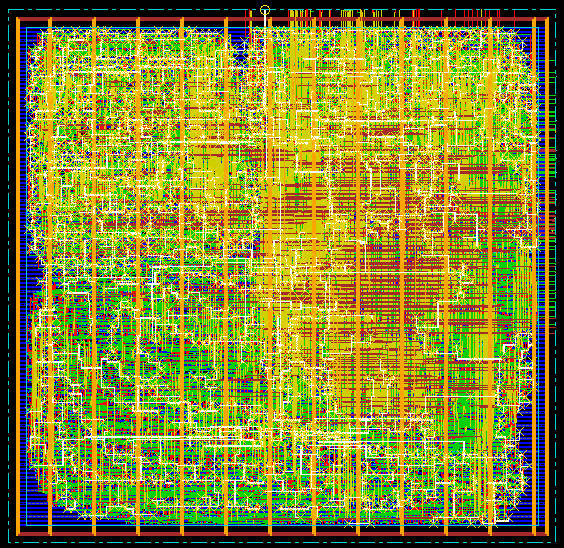
\includegraphics[width=0.60\linewidth, frame]{images/clocktree.png}
		\captionof{figure}{In white we can see the clock tree.}
		\label{fig:clock_tree}
	\end{figure}

	\subsection*{Is the timing met post CTS ? What is your worst timing path ?}

	\begin{lstlisting}
		encounter 10> report_timing
		Path 1: MET Setup Check with Pin HI_RW_reg[29]/CP 
		Endpoint:   HI_RW_reg[29]/D     (^) checked with  leading edge of 'clk_200MHz'
		Beginpoint: S00MUL7_RM_reg[4]/Q (^) triggered by  leading edge of 'clk_200MHz'



		timeDesign Summary                             
		+--------------------+---------+---------+---------+---------+---------+---------+
		|     Setup mode     |   all   | reg2reg | in2reg  | reg2out | in2out  | clkgate |
		+--------------------+---------+---------+---------+---------+---------+---------+
		|           WNS (ns):|  0.091  |  0.091  |  0.826  |   N/A   |   N/A   |   N/A   |
		|           TNS (ns):|  0.000  |  0.000  |  0.000  |   N/A   |   N/A   |   N/A   |
		|    Violating Paths:|    0    |    0    |    0    |   N/A   |   N/A   |   N/A   |
		|          All Paths:|  6714   |  6697   |  1798   |   N/A   |   N/A   |   N/A   |
		+--------------------+---------+---------+---------+---------+---------+---------+
	\end{lstlisting}




	\subsection*{Maybe an optDesign postCTS will optimize that ? Is it better ?}

	As we can see it is a bit better
	\begin{lstlisting}
		optDesign Final Summary                             
		+--------------------+---------+---------+---------+---------+---------+---------+
		|     Setup mode     |   all   | reg2reg | in2reg  | reg2out | in2out  | clkgate |
		+--------------------+---------+---------+---------+---------+---------+---------+
		|           WNS (ns):|  0.113  |  0.113  |  0.824  |   N/A   |   N/A   |   N/A   |
		|           TNS (ns):|  0.000  |  0.000  |  0.000  |   N/A   |   N/A   |   N/A   |
		|    Violating Paths:|    0    |    0    |    0    |   N/A   |   N/A   |   N/A   |
		|          All Paths:|  6714   |  6697   |  1798   |   N/A   |   N/A   |   N/A   |
		+--------------------+---------+---------+---------+---------+---------+---------+
	\end{lstlisting}

	\subsection*{Now that the clock tree is built, you can check if you meet the timing in hold mode. Run: \texttt{timeDesign -postCTS -hold} Is the timing met in hold mode ?}

	Timing is not met, we will try an optimization for both setup and hold.
	\begin{lstlisting}
		timeDesign Summary                             
		+--------------------+---------+---------+---------+---------+---------+---------+
		|     Hold mode      |   all   | reg2reg | in2reg  | reg2out | in2out  | clkgate |
		+--------------------+---------+---------+---------+---------+---------+---------+
		|           WNS (ns):| -0.176  |  0.037  | -0.176  |   N/A   |   N/A   |   N/A   |
		|           TNS (ns):| -11.026 |  0.000  | -11.026 |   N/A   |   N/A   |   N/A   |
		|    Violating Paths:|   84    |    0    |   84    |   N/A   |   N/A   |   N/A   |
		|          All Paths:|  6714   |  6697   |  1798   |   N/A   |   N/A   |   N/A   |
		+--------------------+---------+---------+---------+---------+---------+---------+
	\end{lstlisting}


	\subsection*{Report the timing in hold mode with the report\_timing command. In order to distinguish the setup
		and hold mode report\_timing uses “early” and “late”. Which one is which one ? Explain.}
	Timing is now met post CTS on holde mode.

	\begin{lstlisting}
		timeDesign Summary                             
		+--------------------+---------+---------+---------+---------+---------+---------+
		|     Hold mode      |   all   | reg2reg | in2reg  | reg2out | in2out  | clkgate |
		+--------------------+---------+---------+---------+---------+---------+---------+
		|           WNS (ns):|  0.001  |  0.037  |  0.001  |   N/A   |   N/A   |   N/A   |
		|           TNS (ns):|  0.000  |  0.000  |  0.000  |   N/A   |   N/A   |   N/A   |
		|    Violating Paths:|    0    |    0    |    0    |   N/A   |   N/A   |   N/A   |
		|          All Paths:|  6714   |  6697   |  1798   |   N/A   |   N/A   |   N/A   |
		+--------------------+---------+---------+---------+---------+---------+---------+


		timeDesign Summary                             
		+--------------------+---------+---------+---------+---------+---------+---------+
		|     Setup mode     |   all   | reg2reg | in2reg  | reg2out | in2out  | clkgate |
		+--------------------+---------+---------+---------+---------+---------+---------+
		|           WNS (ns):|  0.113  |  0.113  |  0.824  |   N/A   |   N/A   |   N/A   |
		|           TNS (ns):|  0.000  |  0.000  |  0.000  |   N/A   |   N/A   |   N/A   |
		|    Violating Paths:|    0    |    0    |    0    |   N/A   |   N/A   |   N/A   |
		|          All Paths:|  6714   |  6697   |  1798   |   N/A   |   N/A   |   N/A   |
		+--------------------+---------+---------+---------+---------+---------+---------+
	\end{lstlisting}

	We didn't found early and late but it is written Hold mode and Setup mode.




	\newpage
	\section{Routing the design: NanoRoute}

	\subsection*{Is the post-route timing met ? No ? Let's optimize the timing, Is the timing better ? Please report the worst timing path. What is it ?}
	Timing were not met. Timing are met after optimisation
	\texttt{setAnalysisMode -analysisType onChipVariation} BEFORE \texttt{optDesign -postRoute}, else error ENCOPT 6080 (Thanks to Quentin).

	\begin{lstlisting}
		timeDesign Summary                             
		+--------------------+---------+---------+---------+---------+---------+---------+
		|     Setup mode     |   all   | reg2reg | in2reg  | reg2out | in2out  | clkgate |
		+--------------------+---------+---------+---------+---------+---------+---------+
		|           WNS (ns):|  0.112  |  0.112  |  0.819  |   N/A   |   N/A   |   N/A   |
		|           TNS (ns):|  0.000  |  0.000  |  0.000  |   N/A   |   N/A   |   N/A   |
		|    Violating Paths:|    0    |    0    |    0    |   N/A   |   N/A   |   N/A   |
		|          All Paths:|  6714   |  6697   |  1798   |   N/A   |   N/A   |   N/A   |
		+--------------------+---------+---------+---------+---------+---------+---------+
	\end{lstlisting}

	Worst path :

	\begin{lstlisting}
		Path 1: MET Setup Check with Pin HI_RW_reg[30]/CP 
		Endpoint:   HI_RW_reg[30]/D     (v) checked with  leading edge of 'clk_200MHz'
		Beginpoint: S00MUL7_RM_reg[4]/Q (v) triggered by  leading edge of 'clk_200MHz'
		Analysis View: setup
		Other End Arrival Time          0.261
		- Setup                         0.173
		+ Phase Shift                   5.000
		= Required Time                 5.088
		- Arrival Time                  4.976
		= Slack Time                    0.112
	\end{lstlisting}

	The worst path is inside the multiplier.


	\newpage
	\section{Adding filler cells}

	\subsection*{What is a filler cell ? Why do we need it ?}
	The design rules tell us that there is a need to have continuity between N-well, P-well and Power continuity. If not, cells need to be spaced farther apart. It will be a loss of space.
	Moreover the wells need to be tied to a single global VDD/VSS. Thus,  all the wells of standard cells have to be tied to maintain continuity. It is impossible for a design to fill 100\% of the die with only regular cells. Filler cells are used to fill this space. They reduce DRC violation and help maintain power rail connection continuity.
	\footnote{\url{https://www.quora.com/Why-do-we-use-filler-cells-for-N-well-continuity}}

	\subsection*{Choose “Place > Physical Cells > Add Filler”. Why do call these cells “physical cells” ?}

	\begin{figure}[h!]
		\centering
		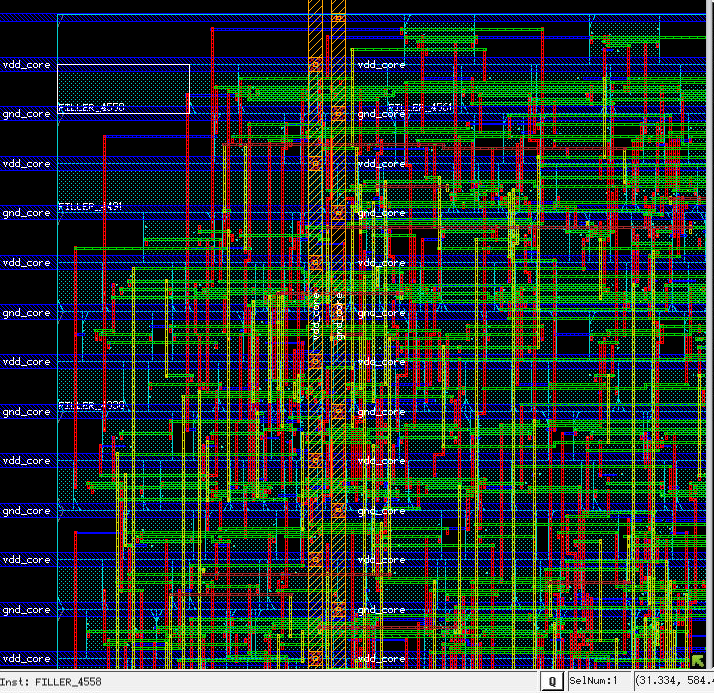
\includegraphics[width=0.60\linewidth, frame]{images/fillercell.png}
		\captionof{figure}{Here we can see a filler cell inside the design. It is called physical cell because they physically take some place on the design.}
		\label{fig:filler_cell}
	\end{figure}

	\begin{lstlisting}
		encounter 14> *INFO: Adding fillers to top-module.
		*INFO:   Added 10 filler insts (cell FILLER2V5CAP64 / prefix FILLER).
		...
		*INFO: Total 4613 filler insts added - prefix FILLER (CPU: 0:00:00.1).
		For 4613 new insts, *** Applied 2 GNC rules (cpu = 0:00:00.0)
		Saving Drc markers ...
		... 0 markers are saved ...
		*INFO: Checking for DRC violations on added fillers.
		...
		*INFO: Iteration 0-#5, Found 0 DRC violation  (real: 0:00:00.0).
		...
		... 0 markers are loaded ...
		*INFO: End DRC Checks. (real: 0:00:04.0 ).
		*INFO: Replaced 175 fillers which had DRC vio's, with 395 new fillers.
	\end{lstlisting}

	\newpage
	\section{Power Rail Analysis}

	It does not work.But I found a course that explain the whole flow\footnote{\url{http://www.ee.ncu.edu.tw/~jfli/vlsidi/lecture/SOC_Encounter.pdf}}
	\begin{lstlisting}
		Rail Analysis is unsuccessful due to errors. 

		Finished Rail Analysis at 20:08:37 02/23/2020 (cpu=0:00:00, real=0:00:01, peak mem=1083.01MB)
		Current Power Analysis resource usage: (total cpu=0:48:36, real=3:48:48, mem=1083.01MB)
		voltus_rail exited unsuccessfully.
		**ERROR: (PRL-387):	"Rail Analysis" failed to finish successfully.
		**ERROR: (EMS-19):	emsIssueMsg failed because the message number 1 does not exist in the catalog file /users/soft/opus/Linux/EDI-13.24.026/share/cdssetup/errormessages/fe/vts.msg.
		Update the catalog file with correct data and re-register the message catalog.
		**ERROR: (VOLTUS-5003):	Net/Group-Net '' does not exist in the design 'MIPS_32_1P_MUL_DIV'. Use always-on net name as the group-net name.
		**ERROR: (VOLTUS-5062):	You must load the state directory before plotting 'ir'.
		**ERROR: **ERROR: (VOLTUS_ERA-2395):	Check error messages in log file.
	\end{lstlisting}

	\begin{figure}[h!]
		\centering
		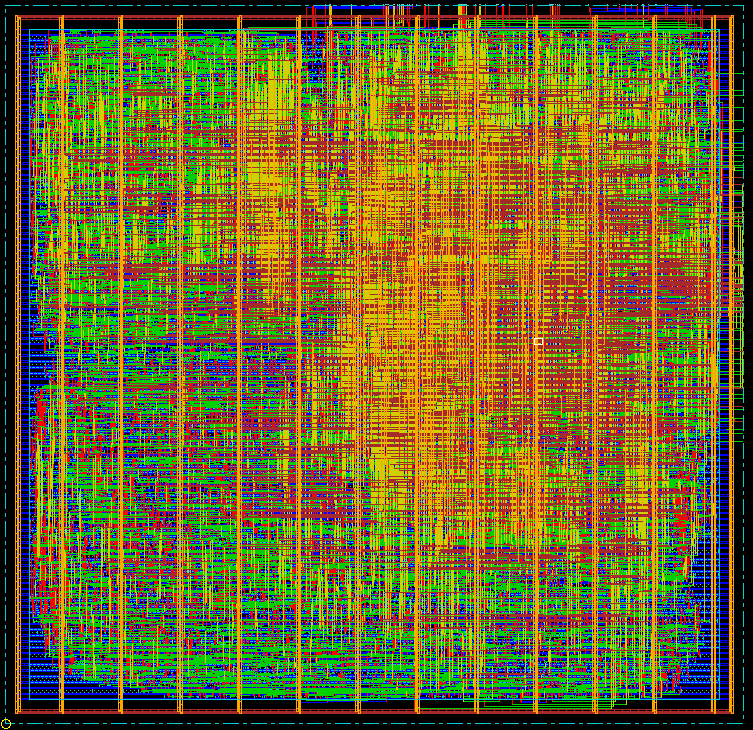
\includegraphics[width=0.60\linewidth, frame]{images/endresult.png}
		\captionof{figure}{Ending result.}
		\label{fig:ending}
	\end{figure}

	\newpage
	\bibliographystyle{IEEEtran}
	\bibliography{biblio}


	\newpage
	\addcontentsline{toc}{chapter}{\listfigurename}
	\listoffigures



	\newpage
	\chapter{Annexe}
	\section{Glossary :}

	\begin{itemize}
		\item EDA : Electronic design automation
		\item DFT : Design For Test %TODO
			%integrated cells for ATPG, Boundary Scan...
		\item CTS : Clock Tree Synthesys : %TODO
		\item STA : Static Timing Analysis  %TODO operates independently of characterization reading both a Verilog netlist and multiple timing 
		\item DRC : Design Rule Check %TODO
		\item LVS : Logical Vs Schematic %TODO extraction of circuit
		\item IC : Integrated Circuit
		\item PCB : Printed Circuit Board
		\item Plot/Pad : %TODO
		\item FP : Floor Planing %TODO (guide the tool)
		\item ATPG : Automatic Test Pattern generation
		\item stuck-at fault : is a fault model for ATPG %TODO
		\item PVT : Process Voltage Temperature %TODO?
		\item Fanout : how much cells my signal can attack without being degraded
		\item .lib : LIBerty : Technology library source files containing all required information for synthesis and static timing analysis
		\item library max (WC=Worst Case) : The timing in this kind of library are the longest (Max path/Max Data path). They are used for setup analysis. 
		\item library min (BC=Best Case) : The timing in the kind of library are the shortest (Min path/Min Data path). They are used for hold analysis.

		\item WNS : Worst negative slack : The longest path in the design
		\item TNS : Total Negative Slack : The Sum of all the longest path in the design
		\item WLM : Wire-Load Model : Statistical Model that \item WHS : Worst Hold Slack (<=>WNS)
		\item THS : Total Hold Slack (<=>TNS)
		\item WPWS : Worst Pulse Width Slack
		\item TPWS : Total Pulse Width Slack
		\item DC : Design Compiler
		\item DCP : Design Compiler Physical
		\item RC : RTL Compiler
		\item RCP : RTL Compiler Physical
		\item SS : Setup Slack : Real time between data latch arrival and clock latch edge, less setup timing. To be TC, all SS must be positive or void.
		\item HS : Hold Slack : Real time between end of data established and end of hold timing. To be TC, all HS must be positive or void.
		\item CDC : Clock Domain Crossing
		\item GDSII : Graphic Database System II
		\item PnR : Place .\& Route

			%\item test at speed : %TODO
		\item floor planning : Macro planing did by human to help EDA tool
			%\item power planning :
		\item spare cells : set of logic cells 
		\item ECO : Engineering Change Order : using of spare cells to prevent any change in design after generated lithographic photomasks, its use to reduced the cost of a design error detecting in back-end flow 
		\item Boundary Scan : 
		\item JTAG : Join Test Action Group :
		\item Trial Route : quick route to predict congestion route, is without fixing DRC or LVS violation
		\item Timing Met
		\item Signoff : Abstract to real, generating GDSII

		\item LEF : Layer Exchange Format : Its a lite physical library for abstract model different from library used to GDSII
		\item SDC : Synopsis Design Constraints : Define timing constraints like input delay, output delay, clock
		\item Shmoo plots ("excel" table)

	\end{itemize}
\end{document}
